\documentclass[conference]{IEEEtran}

\usepackage[utf8]{inputenc}
\usepackage[T1]{fontenc}
\usepackage[brazilian]{babel}
\usepackage{cite}
\usepackage{graphicx}
\usepackage{amsmath}
\usepackage{amssymb}
\usepackage{algorithm}
\usepackage{algpseudocode}
\usepackage{array}
\usepackage{booktabs}
\usepackage{multirow}
\usepackage{url}

\addto\captionsbrazilian{%
  \renewcommand\refname{Referências}%
  \renewcommand{\abstractname}{Resumo}%
  \renewcommand{\tablename}{Tabela}%
  \renewcommand{\figurename}{Figura}%
}
\makeatletter
\renewcommand{\fnum@figure}{\figurename~\thefigure}
\renewcommand{\fnum@table}{\tablename~\thetable}
\makeatother
\floatname{algorithm}{Algoritmo}

\hyphenation{op-tical net-works semi-conduc-tor auto-en-cod-er auto-en-cod-ers ad-ver-sa-ri-al}

\begin{document}

\title{Reprodução e Análise de Robustez de Denoising Autoencoders contra Exemplos Adversariais em Sistemas de Detecção de Intrusão em Redes}

\author{\IEEEauthorblockN{1\textsuperscript{st} Gabriel Marques de Albuquerque}
\IEEEauthorblockA{\textit{Centro de Informática - UFPE} \\
Recife, Brasil \\
gma5@cin.ufpe.br}
\and
\IEEEauthorblockN{2\textsuperscript{nd} Guilherme Lopes Pereira}
\IEEEauthorblockA{\textit{Centro de Informática - UFPE} \\
Recife, Brasil \\
glp3@cin.ufpe.br}
\and
\IEEEauthorblockN{3\textsuperscript{rd} Pedro Vasconcelos de Menezes Case}
\IEEEauthorblockA{\textit{Centro de Informática - UFPE} \\
Recife, Brasil \\
pvmc@cin.ufpe.br}
\and
\IEEEauthorblockN{4\textsuperscript{th} Tomé da Costa Lima}
\IEEEauthorblockA{\textit{Centro de Informática - UFPE} \\
Recife, Brasil \\
tcl@cin.ufpe.br}
}

\maketitle

\begin{abstract}
A evolução contínua em volume, diversidade e sofisticação dos ataques cibernéticos exige o desenvolvimento de Sistemas de Detecção de Intrusão em Redes capazes de identificar ameaças inéditas sob baixas taxas de falsos alertas.
Diante da incapacidade dos sistemas tradicionais baseados em assinaturas para detectar ataques de dia zero, detectores de anomalias não supervisionados fundamentados em redes neurais profundas têm sido amplamente investigados.
Entretanto, estudos recentes demonstram que tais modelos sofrem tanto de supergeneralização na reconstrução de tráfego quanto de severa vulnerabilidade a exemplos adversariais, nos quais um atacante perturba atributos de tráfego de modo a evadir a detecção sem violar a semântica dos protocolos de rede.
Este trabalho realiza a reprodução experimental, a auditoria metodológica e a avaliação de generalização do método de Reconstrução a partir de Observação Parcial e de sua variante aprimorada com agregação por soma de mínimos por grupo, propostos originalmente para elevar a robustez de detectores de anomalias baseados em autoencoders de remoção de ruído.
Os experimentos conduzidos sobre o conjunto de dados de referência nas granularidades de fluxos e de pacotes confirmam a alta fidelidade da reprodução em cenário normal, atingindo taxas médias de detecção de 25,25\% em fluxos e de 34,72\% em pacotes sob taxa de falsos positivos de 1\%, além de preservar a detecção acima da taxa de falsos positivos de 10\% em 8 de 11 ataques de fluxo e em 10 de 11 ataques de pacotes no cenário adversarial.
Paralelamente, a investigação do protocolo original revela limitações metodológicas importantes ligadas ao viés de amostragem temporal e à variância da reavaliação estocástica com máscara única.
Por fim, a aplicação da metodologia a um conjunto adicional de fluxos de Internet das Coisas evidencia que o ganho proporcionado pela agregação de observações parciais se mantém fora do domínio original, mas que a eficácia da evasão adversarial é fortemente dependente das características estatísticas do conjunto de dados.
Complementarmente, o trabalho propõe duas regras de alocação de máscaras por amostra, motivadas pelo custo de cem passagens pelo autoencoder por amostra no RePO+: uma cascata \textit{cheap-first}, que resolve a amostra com um prefixo de dez máscaras e só recorre ao ensemble completo quando o escore barato não é conclusivo, e uma decisão sequencial com parada antecipada por intervalo de confiança.
A cascata reduz o custo de cem para 60,80 máscaras por amostra, uma redução de 39,2\%, preserva exatamente a taxa de detecção do RePO+ completo e mantém taxa de contorno adversarial de 0,25\%; a decisão sequencial reduz o custo em 94,7\% com 99,93\% de concordância com a decisão completa, ao preço de 1,2 ponto percentual de detecção média, e sua avaliação adversarial está em curso.
\end{abstract}

\IEEEpeerreviewmaketitle

\section{Introdução}

O crescimento contínuo das ameaças cibernéticas em escala, diversidade e complexidade tem provocado impactos severos a indivíduos, organizações e infraestruturas críticas, abrangendo desde perdas financeiras bilionárias até interrupções em sistemas de distribuição de energia \cite{symantec2019, icscert2016, kumar2017}.
Nesse cenário, os Sistemas de Detecção de Intrusão em Redes (NIDS, do inglês \textit{Network Intrusion Detection Systems}) constituem um elemento essencial na linha de defesa para monitorar e identificar atividades maliciosas.
Com o avanço de paradigmas como Redes Definidas por Software (SDN), Virtualização de Funções de Rede (NFV), serviços de segurança nativos em nuvem e telemetria programável no plano de dados, tornou-se viável inspecionar de maneira centralizada o tráfego que atravessa os pontos de entrada e comutação da rede \cite{ahmad2015, lee2017}.
Todavia, os NIDS tradicionais baseados em assinaturas mostram-se insuficientes frente ao panorama atual de ameaças, pois dependem de padrões previamente conhecidos e são incapazes de detectar ataques de dia zero (\textit{zero-day attacks}) ou variantes polimórficas de intrusão \cite{khraisat2019}.

Para superar a rigidez das assinaturas, a literatura recente passou a empregar técnicas de aprendizado de máquina e aprendizado profundo na construção de NIDS baseados em detecção de anomalias \cite{alqatf2018, yu2017, yin2018, malaiya2018, mirsky2018, zong2018, zenati2018, chalapathy2019}.
Esses sistemas são treinados de forma não supervisionada exclusivamente sobre tráfego benigno, aprendendo um perfil de normalidade da rede.
Na fase de inferência, cada pacote ou fluxo observado recebe um escore de dissimilaridade em relação ao perfil aprendido; caso esse escore ultrapasse um limiar de decisão predefinido, o tráfego é classificado como malicioso.
Para que um detector de anomalias seja operacionalmente viável em redes reais de alto volume, esse limiar deve ser calibrado de modo a garantir uma taxa de falsos positivos ($\text{FPR}$, do inglês \textit{False Positive Rate}) extremamente reduzida.
Caso contrário, em virtude da falácia da taxa base (\textit{base-rate fallacy}) \cite{axelsson2000}, o volume absoluto de alertas falsos gerados pelo tráfego legítimo inviabiliza a triagem humana por especialistas de segurança.

Apesar do potencial dos NIDS baseados em aprendizado profundo, investigações recentes demonstraram que sua capacidade de detecção apresenta duas fragilidades estruturais graves \cite{hashemi2019, aiken2019, hashemi2020}.
A primeira reside no problema de supergeneralização (\textit{over-generalization}) em modelos reconstrutivos convencionais, como \textit{autoencoders} treinados com observação completa dos atributos de entrada \cite{mirsky2018}: devido à elevada capacidade representacional das redes neurais, o modelo aprende transformações próximas à identidade e passa a reconstruir amostras anômalas — nunca vistas no treinamento — com erro tão baixo quanto o de amostras benignas, degradando drasticamente a taxa de detecção ($\text{TPR}$, do inglês \textit{True Positive Rate}, ou taxa de verdadeiros positivos) sob baixas taxas de falsos alertas.
A segunda fragilidade decorre da natureza determinística desses modelos durante a inferência, o que os torna altamente suscetíveis a ataques de evasão por exemplos adversariais \cite{biggio2013, szegedy2013, hashemi2019}.
Nesses ataques, o adversário manipula sutilmente o tráfego malicioso — por exemplo, alterando intervalos entre pacotes, fragmentando cargas úteis ou injetando pacotes sintéticos — para reduzir o escore de anomalia abaixo do limiar de detecção sem comprometer a funcionalidade do ataque nem violar os protocolos de comunicação subjacentes.

Diante dessas limitações, Hashemi e Keller \cite{hashemi2020} propuseram o mecanismo \textit{Reconstruction from Partial Observation} (RePO) e sua versão estendida RePO+ para a construção de NIDS não supervisionados mais precisos e resilientes a exemplos adversariais.
A abordagem substitui a observação integral da entrada pelo treinamento de \textit{Denoising Autoencoders} (DAE) \cite{vincent2008} combinados com máscaras binárias aleatórias que ocultam a maior parte dos atributos de entrada.
Ao exigir que a rede neural gere os atributos ausentes a partir de uma visão parcial da amostra, o método impede a supergeneralização e amplia a separação entre os erros de reconstrução de tráfego benigno e malicioso.
Adicionalmente, na inferência do RePO+, cada amostra é avaliada paralelamente sob $100$ máscaras aleatórias distintas divididas em $5$ grupos, somando-se os erros mínimos de cada grupo.
Essa estratégia atenua o impacto de máscaras que ocultem atributos essenciais em amostras legítimas e introduz não-determinismo na inferência, dificultando a transferência de exemplos adversariais gerados em cópias locais do modelo pelo atacante.

Sob essa ótica, este trabalho investiga a reprodutibilidade científica, a validade metodológica e a capacidade de generalização do sistema RePO/RePO+ em diferentes representações e domínios de tráfego de rede.
As principais contribuições deste trabalho são:

\begin{itemize}
    \item Reproduzir integralmente e validar empiricamente os experimentos do artigo de referência \cite{hashemi2020} para detecção de intrusão baseada em fluxos e em pacotes sobre o conjunto de dados CICIDS2017 \cite{sharafaldin2018}, avaliando os modos RePO e RePO+ tanto no cenário normal ($\text{FPR} = 0{,}01$) quanto sob ataques adversariais ($\text{FPR} = 0{,}10$);
    \item Realizar uma auditoria metodológica e estatística rigorosa do protocolo experimental de referência, identificando e quantificando o impacto do viés de amostragem temporal na seleção sequencial de instâncias de ataque, da variância estocástica associada à reavaliação por máscara única e da desproporção amostral em classes minoritárias;
    \item Estender a avaliação do método RePO/RePO+ e do ataque adversarial de fluxo para um novo conjunto de dados de tráfego de Internet das Coisas (CIC-ToN-IoT), demonstrando que a vantagem da agregação por mínimos por grupo se mantém em um novo domínio, ao passo que a transferibilidade e o sucesso do ataque adversarial dependem fortemente da distribuição dos atributos e da escala dos escores de reconstrução;
    \item Propor e avaliar duas regras de alocação de máscaras por amostra que reduzem o custo de inferência do RePO+ sem substituir a função de decisão na região difícil do espaço de entrada: uma cascata \textit{cheap-first} com estágio barato de dez máscaras, que reduz o custo em $39{,}2\%$ preservando exatamente a detecção do detector completo e mantendo taxa de contorno adversarial de 0,25\%, e uma decisão sequencial com parada antecipada por intervalo de confiança, que reduz o custo em $94{,}7\%$ ao preço de $1{,}2$ ponto percentual de detecção média.
\end{itemize}

\section{Trabalhos relacionados}

A literatura relacionada a este estudo divide-se em duas vertentes complementares: o projeto de detectores de anomalias não supervisionados baseados em aprendizado profundo para tráfego de rede e a formulação de ataques de evasão adversarial contra sistemas de detecção de intrusão.

\subsection{Detecção de Anomalias em Redes com Aprendizado Profundo}

O uso de arquiteturas de aprendizado profundo para detecção de anomalias em redes busca contornar a dependência de dados rotulados de ataques e permitir a identificação de ameaças inéditas \cite{chalapathy2019, khraisat2019}.
Em linhas iniciais de investigação, Yu et al. \cite{yu2017} propuseram o empilhamento de \textit{autoencoders} convolucionais dilatados para extrair representações hierárquicas de tráfego de forma não supervisionada, enquanto Al-Qatf et al. \cite{alqatf2018} combinaram \textit{autoencoders} esparsos para redução de dimensionalidade com classificadores baseados em Máquinas de Vetores de Suporte (SVM).
De modo similar, Yin et al. \cite{yin2018} exploraram Redes Adversariais Generativas (GANs) para aprimorar a detecção de \textit{botnets}, e Malaiya et al. \cite{malaiya2018} avaliaram empiricamente arquiteturas variacionais e recorrentes na detecção de anomalias de rede.
Contudo, grande parte dessas abordagens iniciais ainda depende de etapas supervisionadas para classificação final ou foi validada em conjuntos de dados legados que não refletem a diversidade do tráfego moderno.

Entre os detectores estritamente não supervisionados considerados estado da arte no nível de pacotes, destaca-se o Kitsune, proposto por Mirsky et al. \cite{mirsky2018}.
O Kitsune opera de maneira online extraindo estatísticas incrementais de fluxo a partir de cabeçalhos de pacotes e distribuindo os atributos resultantes em um conjunto (\textit{ensemble}) de pequenos \textit{autoencoders} de três camadas, cujos erros de reconstrução alimentam um \textit{autoencoder} agregador final (variante Kitsune-AE) ou um estimador de densidade baseado em Modelo de Mistura Gaussiana (variante Kitsune-GMM).
Embora apresente baixa sobrecarga computacional, o Kitsune reconstrói cada vetor a partir da observação integral de seus atributos.
Consequentemente, a rede tende a sofrer de supergeneralização, produzindo erros de reconstrução reduzidos mesmo para pacotes maliciosos e resultando em baixa sensibilidade quando o limiar operacional é restrito a uma taxa de falsos positivos de $1\%$ \cite{hashemi2020}.

No contexto de detecção baseada em fluxos, Zong et al. \cite{zong2018} introduziram o \textit{Deep Autoencoding Gaussian Mixture Model} (DAGMM), que acopla um \textit{undercomplete autoencoder} profundo a uma sub-rede de mistura gaussiana -- que faz a estimativa -- treinada conjuntamente fim a fim.
O modelo concatena a representação latente de baixa dimensão com métricas de erro de reconstrução para calcular a energia amostral de cada fluxo, classificando como anômalas as instâncias de alta energia.
Apesar de mitigar ótimos locais decorrentes do desacoplamento entre redução de dimensionalidade e estimativa de densidade, o DAGMM permanece determinístico e apresenta capacidade limitada para separar ataques complexos de fluxos benignos sob baixas taxas de falsos alertas.

Outra abordagem de destaque para dados tabulares e fluxos de rede é o detector baseado em Redes Adversariais Generativas Bidirecionais (BiGAN), proposto por Zenati et al. \cite{zenati2018}.
Diferentemente de GANs convencionais que exigem otimização iterativa custosa para mapear uma amostra ao espaço latente, a arquitetura BiGAN treina simultaneamente um codificador e um gerador, definindo o escore de anomalia como uma soma ponderada entre o erro de reconstrução das características e o erro de discriminação conjunta.
Ainda que alcance inferência rápida e desempenho superior ao DAGMM em cenários normais de fluxo, a arquitetura BiGAN compartilha a vulnerabilidade estrutural de modelos determinísticos frente a perturbações adversariais direcionadas \cite{hashemi2019, hashemi2020}.

\subsection{Exemplos Adversariais contra Sistemas de Detecção de Intrusão}

A vulnerabilidade de modelos de aprendizado de máquina e redes neurais profundas a exemplos adversariais em tempo de teste foi inicialmente estabelecida por Biggio et al. \cite{biggio2013} e Szegedy et al. \cite{szegedy2013}, expandindo-se rapidamente para domínios como visão computacional \cite{sharif2016, eykholt2018}, reconhecimento de voz \cite{carlini2018} e detecção de \textit{malware} \cite{grosse2017}.
Diferentemente do domínio de imagens — no qual cada pixel pode ser perturbado continuamente dentro de uma bola de norma limitada —, a geração de exemplos adversariais no tráfego de rede impõe restrições severas de domínio: as perturbações não podem corromper cabeçalhos de protocolo, violar correlações matemáticas entre atributos derivados (como médias, taxas de bytes por segundo e contadores de pacotes) nem anular a carga maliciosa do ataque.

Aiken e Scott-Hayward \cite{aiken2019} investigaram ataques adversariais contra um NIDS implantado em ambiente SDN, demonstrando que um atacante pode evadir a detecção de ataques de negação de serviço distribuída (DDoS) mediante a combinação de aumento do tamanho de carga útil, redução da taxa de transmissão e injeção de fluxos simétricos forjados.
Todavia, a metodologia proposta restringiu-se a ataques volumétricos específicos de DDoS e a classificadores supervisionados sob condições restritas de fluxo.

Para estabelecer uma avaliação abrangente e realista, Hashemi et al. \cite{hashemi2019} formularam um modelo de ameaça geral para NIDS baseados em anomalias tanto na granularidade de fluxos quanto na de pacotes.
No nível de fluxos, os autores categorizaram os atributos em grupos conforme sua mutabilidade física e semântica, projetando um algoritmo de otimização restrita que recalcula atributos dependentes a cada passo de gradiente.
No nível de pacotes, demonstraram que a combinação de operações válidas de rede — atraso temporal entre pacotes (\textit{delay}), fragmentação de pacotes (\textit{splitting}) e injeção de pacotes sintéticos ignorados pelo hospedeiro vítima — reduz drasticamente a eficácia de detectores como Kitsune, DAGMM e BiGAN.
Contudo, esse trabalho concentrou-se na construção do ataque e no diagnóstico da vulnerabilidade dos NIDS existentes, sem apresentar uma arquitetura defensiva robusta.

Com base no alicerce teórico dos \textit{Denoising Autoencoders} de Vincent et al. \cite{vincent2008}, Hashemi e Keller \cite{hashemi2020} propuseram o método RePO/RePO+ (artigo de referência deste relatório).
Ao combinar reconstrução a partir de observação parcial com agregação estocástica de múltiplas máscaras aleatórias na inferência, os autores demonstraram ganhos expressivos de detecção sobre Kitsune, DAGMM e BiGAN tanto em operação normal quanto sob o modelo de ameaça adversarial de Hashemi et al. \cite{hashemi2019}.
A Tabela~\ref{tab:trabalhos-relacionados} sintetiza os principais trabalhos relacionados, destacando os métodos empregados, suas vantagens e suas limitações.

\begin{table*}[!t]
\centering
\caption{Síntese comparativa dos principais trabalhos relacionados em detecção de intrusão por anomalias e robustez adversarial.}
\label{tab:trabalhos-relacionados}
\begin{tabular}{@{}>{\raggedright\arraybackslash}p{2.8cm}>{\raggedright\arraybackslash}p{3.6cm}>{\raggedright\arraybackslash}p{5.2cm}>{\raggedright\arraybackslash}p{5.2cm}@{}}
\toprule
\textbf{Trabalho} & \textbf{Método} & \textbf{Vantagens / Contribuições} & \textbf{Desvantagens / Limitações} \\
\midrule
Mirsky et al. (Kitsune) \cite{mirsky2018} & Conjunto (\textit{ensemble}) de \textit{autoencoders} (ou GMM) sobre estatísticas incrementais de pacotes. & Processamento online leve sem necessidade de supervisão; extração automática de agrupamentos de atributos. & Supergeneralização por observação completa da entrada; baixa detecção em $\text{FPR}=0{,}01$; altamente vulnerável a evasão adversarial determinística. \\
\addlinespace
Zong et al. (DAGMM) \cite{zong2018} & \textit{Autoencoder} profundo acoplado fim a fim a uma rede estimadora de Mistura Gaussiana. & Otimização conjunta do espaço latente e da densidade; evita ótimos locais na compressão de atributos de fluxo. & Inferência determinística; baixa sensibilidade sob limiares estritos de falsos alertas; suscetível a ataques adversariais em fluxos. \\
\addlinespace
Zenati et al. (BiGAN) \cite{zenati2018} & Rede Adversarial Generativa Bidirecional com codificador e gerador conjuntos. & Inferência rápida no espaço latente; combina erro de reconstrução e discriminação para detecção em fluxos. & Instabilidade de treinamento inerente a arquiteturas GAN; comportamento determinístico facilita evasão adversarial por gradiente. \\
\addlinespace
Aiken e Scott-Hayward \cite{aiken2019} & Manipulação heurística de atributos de tráfego (carga útil, taxa e simetria) em redes SDN. & Demonstra a viabilidade prática de evasão adversarial contra NIDS em ambientes definidos por software. & Escopo restrito a ataques DDoS específicos; não modela restrições gerais de múltiplos protocolos nem propõe defesa robusta. \\
\addlinespace
Hashemi et al. \cite{hashemi2019} & Otimização adversarial restrita ao domínio em nível de fluxo e transformações válidas em pacotes. & Formulação sistemática de ataques adversariais que preservam a semântica de rede contra NIDS estado da arte. & Atua exclusivamente no diagnóstico ofensivo da vulnerabilidade; não propõe mecanismo de defesa para os detectores avaliados. \\
\addlinespace
Hashemi e Keller (RePO / RePO+) \cite{hashemi2020} & \textit{Denoising Autoencoders} com mascaramento aleatório parcial e agregação por mínimos por grupo. & Mitiga a supergeneralização; estocasticidade de $100$ máscaras eleva a detecção normal e a robustez adversarial em fluxos e pacotes. & Custo computacional de inferência ampliado pelas múltiplas máscaras; avaliação original sujeita a viés de amostragem temporal e avaliada em único domínio. \\
\bottomrule
\end{tabular}
\end{table*}

\section{Modelo de ameaça}

O modelo de ameaça adotado neste trabalho segue a formulação de ataques de evasão em tempo de teste proposta por Hashemi et al. \cite{hashemi2019} e empregada na avaliação do sistema de referência \cite{hashemi2020}.
Considera-se um ambiente de rede monitorado por um NIDS baseado em detecção de anomalias não supervisionada, posicionado em um ponto de agregação ou comutação para inspecionar o tráfego bidirecional (no nível de fluxos) ou unidirecional/sequencial (no nível de pacotes).

\subsection{Premissas de Conhecimento, Capacidades e Restrições do Atacante}

Assume-se um adversário com conhecimento em regime de caixa-branca (\textit{white-box}) acerca dos componentes estáticos do detector: o atacante conhece o conjunto de atributos monitorados, os vetores de normalização mínimo ($\mathbf{x}_{\min}$) e máximo ($\mathbf{x}_{\max}$) extraídos do conjunto de treinamento, a arquitetura e os parâmetros treinados $\theta$ da rede neural reconstrutiva $f_{\theta}$, bem como o limiar operacional de detecção $\tau$ calibrado para uma taxa de falsos positivos predefinida ($\text{FPR} = 0{,}10$ no cenário adversarial).
Contudo, quando o detector vítima emprega inferência estocástica com mascaramento aleatório, o atacante não possui acesso à \textit{seed} pseudoaleatória nem às realizações exatas das máscaras binárias sorteadas pelo detector no instante em que o tráfego atravessa a rede.
Dessa forma, o adversário precisa otimizar as perturbações utilizando uma cópia local do detector (com sua própria amostragem independente de máscaras) e transmitir o tráfego resultante para avaliação pelo NIDS vítima.

O escopo de ameaças abrange múltiplas famílias de ataques de rede: negação de serviço na camada de aplicação e transporte (\textit{DoS Hulk}, \textit{DoS GoldenEye}, \textit{DoS Slowloris} e \textit{DoS Slowhttptest}), negação de serviço distribuída (\textit{DDoS}), reconhecimento por varredura de portas (\textit{PortScan}), força bruta em serviços de transferência e administração remota (\textit{FTP-Patator} e \textit{SSH-Patator}), comunicação de comando e controle (\textit{Botnet}), exploração de vulnerabilidades e exfiltração (\textit{Heartbleed} e \textit{Infiltration}), além de vetores modernos em ambientes de Internet das Coisas (\textit{cross-site scripting}, injeção, \textit{ransomware}, \textit{backdoor} e interceptação \textit{man-in-the-middle}).

Diferentemente de domínios contínuos como imagens, o atacante está submetido a três restrições de domínio estritas ao manipular uma amostra maliciosa $\mathbf{x}$:
\begin{enumerate}
    \item \textbf{Preservação funcional do ataque:} a carga maliciosa e a semântica da exploração não podem ser removidas ou corrompidas;
    \item \textbf{Controlabilidade unilateral:} o atacante controla apenas os pacotes que transmite (sentido \textit{forward}), não podendo alterar diretamente os pacotes de resposta gerados pelo hospedeiro vítima (sentido \textit{backward});
    \item \textbf{Consistência matemática e de protocolo:} cabeçalhos de pacotes devem permanecer sintaticamente válidos e todas as relações determinísticas entre atributos primários, agregados e derivados devem ser preservadas na representação final observada pelo NIDS.
\end{enumerate}

\subsection{Ataque Adversarial Baseado em Fluxos}

Na representação baseada em fluxos, cada conexão é sintetizada por um vetor $\mathbf{x} \in \mathbb{R}^{D}$ com $D = 77$ atributos estatísticos.
Como o vetor de fluxo é computado pelo monitor de rede a partir da sequência de pacotes transmitidos, o atacante não pode perturbar livremente coordenadas arbitrárias de $\mathbf{x}$.
Para garantir validade física e semântica, os $77$ atributos são particionados em quatro grupos funcionais \cite{hashemi2019, hashemi2020}:
\begin{itemize}
    \item \textbf{Atributos fixos (imutáveis):} características fora do controle direto do atacante ou cuja alteração invalidaria o serviço alvo, incluindo a porta de destino e estatísticas exclusivas do fluxo reverso (\textit{backward});
    \item \textbf{Atributos diretamente otimizáveis em níveis hierárquicos:} variáveis controláveis pelo emissor no sentido \textit{forward} (como duração do fluxo, contagens de pacotes, comprimentos de carga útil e tempos inter-chegada), estruturadas em três máscaras binárias progressivas de mutabilidade $\mathbf{v}_1, \mathbf{v}_2, \mathbf{v}_3 \in \{0, 1\}^{D}$ ($\mathcal{M}_1 \subset \mathcal{M}_2 \subset \mathcal{M}_3$), nas quais $\mathbf{v}_1$ habilita apenas atributos primários essenciais, $\mathbf{v}_2$ adiciona estatísticas intermediárias de janelas e cabeçalhos, e $\mathbf{v}_3$ libera atributos agregados de atividade e ociosidade caso os níveis anteriores não alcancem evasão;
    \item \textbf{Atributos restritos por monotonicidade e integridade:} variáveis que representam valores mínimos observados no fluxo (restritas ao intervalo $[0, x_j]$), valores máximos e contadores de \textit{flags} TCP (restritos a valores $\ge x_j$), e atributos discretos cujo domínio pertence a $\mathbb{Z}_{\ge 0}$;
    \item \textbf{Atributos dependentes e duplicados:} $17$ grandezas compostas (taxas de bytes e pacotes por segundo, razões entre direções, médias de tamanhos de pacotes e de tempos inter-chegada, e comprimentos totais de cabeçalhos) e $4$ atributos de subfluxo que espelham contagens primárias, todos recalculados analiticamente após qualquer alteração nos atributos primários.
\end{itemize}

Seja $\tilde{\mathbf{x}}$ a representação normalizada de um fluxo malicioso $\mathbf{x}$ segundo os limites do conjunto de treinamento:
\begin{equation}
\tilde{\mathbf{x}} = \frac{\mathbf{x} - \mathbf{x}_{\min}}{\mathbf{x}_{\max} - \mathbf{x}_{\min} + \epsilon}, \quad \epsilon = 10^{-6}.
\label{eq:norm_fluxo}
\end{equation}
Para uma máscara de mutabilidade $\mathbf{v} \in \{\mathbf{v}_1, \mathbf{v}_2, \mathbf{v}_3\}$, o atacante introduz um vetor modificador contínuo $\boldsymbol{\alpha} \in \mathbb{R}^{D}$ no espaço normalizado, produzindo a amostra candidata $\tilde{\mathbf{x}}_{\text{cand}}(\boldsymbol{\alpha}) = \tilde{\mathbf{x}} + \boldsymbol{\alpha} \odot \mathbf{v}$, onde $\odot$ denota o produto de Hadamard (elemento a elemento).
Para contornar o mascaramento aleatório do detector, a cada passo de otimização o atacante sorteia $M = 100$ máscaras binárias independentes $\mathbf{m}_i \in \{0, 1\}^{D}$ e minimiza a função objetivo dada pela soma dos erros quadráticos médios de reconstrução em relação a $\boldsymbol{\alpha}$:
\begin{equation}
\mathcal{L}_{\text{adv}}^{\text{fluxo}}(\boldsymbol{\alpha}) = \sum_{i=1}^{M} \frac{1}{D} \left\| f_{\theta}\!\left(\tilde{\mathbf{x}}_{\text{cand}}(\boldsymbol{\alpha}) \odot \mathbf{m}_i\right) - \tilde{\mathbf{x}}_{\text{cand}}(\boldsymbol{\alpha}) \right\|_2^2.
\label{eq:loss_adv_fluxo}
\end{equation}

Após cada passo de atualização de $\boldsymbol{\alpha}$ por descida de gradiente adaptativa (Adam), o vetor candidato é desnormalizado para o domínio original e submetido a um operador de projeção determinístico $\mathbf{x}^{\text{adv}} = \Pi_{\mathcal{V}}(\mathbf{x}_{\text{cand}}(\boldsymbol{\alpha}), \mathbf{x})$.
O operador $\Pi_{\mathcal{V}}$ executa sequencialmente: (i) a cópia exata dos atributos primários para seus atributos de subfluxo duplicados; (ii) o truncamento dos atributos mínimos em $[0, x_j]$ e dos atributos máximos e de \textit{flags} em $[x_j, +\infty)$, incrementando o total de pacotes \textit{forward} pelo maior acréscimo de \textit{flags}; (iii) o arredondamento ao inteiro mais próximo de todas as coordenadas discretas; e (iv) a recomputação exata das variáveis derivadas (taxas por segundo, médias de pacotes, médias de intervalos temporais e bytes de cabeçalho).

A busca pelo exemplo adversarial percorre em cascata as máscaras $\mathbf{v}_1, \mathbf{v}_2, \mathbf{v}_3$ e, para cada máscara, quatro configurações de taxa de aprendizado $\eta \in \{0{,}001;\, 0{,}01;\, 0{,}1;\, 1{,}0\}$ com limites respectivos de $\{30, 40, 50, 60\}$ iterações.
Como a avaliação final no NIDS vítima utiliza um novo sorteio estocástico de máscaras, o atacante adota um limiar alvo conservador $\tau_{\text{adv}} = 0{,}8\tau$: o procedimento encerra imediatamente quando o escore local RePO+ satisfaz $S_{\text{RePO+}}(\mathbf{x}^{\text{adv}}) < 0{,}8\tau$, mantendo como solução de contingência a primeira configuração que atingir $S_{\text{RePO+}}(\mathbf{x}^{\text{adv}}) < \tau$.

\subsection{Ataque Adversarial Baseado em Pacotes}

Na granularidade de pacotes, cada amostra de entrada do detector consiste em uma janela deslizante $\mathbf{X} = [\mathbf{x}_1, \mathbf{x}_2, \dots, \mathbf{x}_T]^{\top} \in \mathbb{R}^{T \times D}$ formada por $T = 20$ pacotes consecutivos e $D = 29$ atributos extraídos dos cabeçalhos IP, TCP, UDP e ICMP (incluindo intervalo temporal inter-pacotes $\Delta t$, comprimentos de quadro e de cabeçalho IP, flags, janelas e indicador de direção), na qual $\mathbf{x}_T$ representa o pacote atual sob inspeção.
Como os pacotes $\mathbf{x}_1, \dots, \mathbf{x}_{T-1}$ já transitaram pela rede, eles não podem ser modificados retroativamente.
O atacante dispõe de três transformações válidas de tráfego \cite{hashemi2019}:
\begin{enumerate}
    \item \textbf{Atraso temporal (\textit{Delay}):} adição de um retardo $\delta_{\text{delay}} \in [0, 15]$ segundos ao tempo inter-chegada do pacote atual $\mathbf{x}_T$;
    \item \textbf{Fragmentação (\textit{Splitting}):} redução do comprimento total do pacote $\mathbf{x}_T$ (de tamanho original $L_T$) por uma quantidade $\delta_{\text{split}} \in [-(L_T - 61), 0]$ bytes — respeitando o tamanho mínimo de quadro de $60$ bytes — e transmissão da carga útil restante $\Delta L = L_T - L'_T$ em um pacote subsequente de comprimento $\Delta L + 60$ bytes e intervalo temporal $\Delta t = 0$, o qual é otimizado recursivamente pelo mesmo procedimento;
    \item \textbf{Injeção de pacote sintético (\textit{Injection}):} criação e transmissão de um pacote forjado $\mathbf{p}_{\text{fake}} \in \mathbb{R}^{D}$ limitado ao domínio válido dos cabeçalhos $[\mathbf{p}_{\min}, \mathbf{p}_{\max}]$ e filtrado por uma máscara binária de protocolo $\mathbf{u}_{\text{proto}} \in \{\mathbf{u}_{\text{TCP}}, \mathbf{u}_{\text{UDP}}\}$, mantendo o atributo de viabilidade nulo para que o pacote seja descartado pela pilha de rede do destino sem interferir na sessão.
\end{enumerate}

Quando o pacote atual $\mathbf{x}_T$ é emitido pelo atacante, aplica-se prioritariamente a otimização conjunta de atraso e fragmentação por até $300$ iterações ($\eta = 0{,}1$), minimizando a perda de reconstrução agregada sobre $M = 100$ máscaras análoga à Eq.~\eqref{eq:loss_adv_fluxo} e arredondando os campos de comprimento a cada passo.
Caso a otimização conjunta não reduza o escore RePO+ abaixo de $\tau$ — ou quando o pacote $\mathbf{x}_T$ é um pacote de resposta emitido pelo servidor vítima, sobre o qual o atacante não pode impor atraso ou divisão —, executa-se a operação de injeção.
Na injeção, o pacote sintético $\mathbf{p}_{\text{fake}}$ é inserido imediatamente antes de $\mathbf{x}_T$, dando origem a duas janelas consecutivas observadas pelo NIDS: $\mathbf{X}^{(1)} = [\mathbf{x}_1, \dots, \mathbf{x}_{19}, \mathbf{p}_{\text{fake}}]^{\top}$ e $\mathbf{X}^{(2)} = [\mathbf{x}_2, \dots, \mathbf{x}_{19}, \mathbf{p}_{\text{fake}}, \mathbf{x}_{20}]^{\top}$.
O atacante otimiza $\mathbf{p}_{\text{fake}}$ por até $300$ iterações ($\eta = 0{,}1$) minimizando a soma conjunta dos erros de reconstrução de $\mathbf{X}^{(1)}$ e $\mathbf{X}^{(2)}$, considerando a evasão bem-sucedida somente se ambas as janelas atingirem simultaneamente escore RePO+ inferior ao limiar $\tau$.

\section{Sistema proposto pelo artigo de referência}\label{sec:sistema_referencia}

Para mitigar simultaneamente a supergeneralização de modelos reconstrutivos convencionais e a vulnerabilidade a exemplos adversariais, Hashemi e Keller \cite{hashemi2020} propuseram a arquitetura \textit{Reconstruction from Partial Observation} (RePO) e sua variante aprimorada RePO+.

\subsection{Princípio de Reconstrução a partir de Observação Parcial}

Em um \textit{autoencoder} padrão treinado para minimizar $\|f_{\theta}(\tilde{\mathbf{x}}) - \tilde{\mathbf{x}}\|_2^2$ a partir da observação completa de $\tilde{\mathbf{x}}$, a presença de todos os atributos na entrada permite que redes de alta capacidade aprendam mapeamentos próximos à identidade.
Como consequência, mesmo amostras maliciosas situadas fora da variedade do tráfego benigno são reconstruídas com baixo erro.
Além disso, como o mapeamento $\tilde{\mathbf{x}} \mapsto f_{\theta}(\tilde{\mathbf{x}})$ é inteiramente determinístico, um atacante em caixa-branca calcula gradientes exatos da superfície de decisão para construir exemplos adversariais com mínima perturbação.

O sistema RePO reformula o detector como um \textit{Denoising Autoencoder} (DAE) \cite{vincent2008} submetido a um operador de mascaramento binário estocástico.
Dada uma amostra normalizada $\tilde{\mathbf{x}}$ — seja um vetor de fluxo em $\mathbb{R}^{D}$ ou uma janela temporal de pacotes em $\mathbb{R}^{T \times D}$ —, sorteia-se uma máscara aleatória $\mathbf{m}$ de mesmas dimensões cujas componentes são variáveis de Bernoulli independentes e identicamente distribuídas:
\begin{equation}
m_j = \mathbb{I}\!\left(u_j > p_{\text{mask}}\right), \quad u_j \sim \mathcal{U}(0, 1),
\label{eq:bernoulli_mask}
\end{equation}
onde $\mathbb{I}(\cdot)$ é a função indicadora e $p_{\text{mask}} = 0{,}75$ representa a probabilidade de ocultação de cada atributo.
Assim, apenas $1 - p_{\text{mask}} = 25\%$ dos atributos originais são preservados em média na observação parcial $\tilde{\mathbf{x}}_{\text{parcial}} = \tilde{\mathbf{x}} \odot \mathbf{m}$, enquanto os $75\%$ restantes são substituídos por zero.

Durante o treinamento — realizado de maneira estritamente não supervisionada apenas sobre amostras de tráfego benigno $\mathcal{D}_{\text{train}}$ —, a rede neural recebe a observação parcial $\tilde{\mathbf{x}} \odot \mathbf{m}$, mas é penalizada pelo erro quadrático médio de reconstrução em relação à amostra completa $\tilde{\mathbf{x}}$ (incluindo os $75\%$ de atributos ocultados em média):
\begin{equation}
\mathcal{L}_{\text{DAE}}(\theta) = \mathbb{E}_{\tilde{\mathbf{x}} \sim \mathcal{D}_{\text{train}},\, \mathbf{m}}\!\left[ \frac{1}{d} \left\| f_{\theta}\!\left(\tilde{\mathbf{x}} \odot \mathbf{m}\right) - \tilde{\mathbf{x}} \right\|_2^2 \right],
\label{eq:loss_dae}
\end{equation}
em que $d$ denota o número total de coordenadas da entrada ($d = D = 77$ para fluxos e $d = T \cdot D = 580$ para pacotes).
Para minimizar a Eq.~\eqref{eq:loss_dae}, o modelo não pode simplesmente copiar a entrada; ele é forçado a aprender as dependências estatísticas e estruturais que governam os atributos do tráfego benigno, extrapolando os atributos ausentes a partir do subconjunto visível.
Quando confrontado na inferência com uma amostra de ataque cujas correlações internas divergem do perfil normal, a extrapolação falha nos atributos ocultos, elevando acentuadamente o erro de reconstrução.

\subsection{Arquitetura das Redes Neurais para Fluxos e Pacotes}

O sistema de referência instancia duas arquiteturas distintas de DAEs conforme a granularidade de inspeção do tráfego:
\begin{itemize}
    \item \textbf{Modelo Baseado em Fluxos ($D = 77$):} consiste em uma rede perceptrônica multicamadas totalmente conectada composta por sete camadas densas com função de ativação ReLU ($\text{ReLU}(z) = \max(0, z)$).
    A entrada parcial $\tilde{\mathbf{x}} \odot \mathbf{m} \in \mathbb{R}^{77}$ atravessa seis camadas ocultas sucessivas de $256$ neurônios cada, intercaladas por duas camadas de regularização por \textit{Dropout} com probabilidade de descarte de $0{,}5$ após a terceira e a quinta camadas ocultas (ativas exclusivamente durante o treinamento).
    A sétima camada densa projeta a representação latente de volta para a dimensão original $D = 77$ com ativação ReLU, sendo seguida por um operador de truncamento (\textit{clipping}) ao intervalo $[0, 1]$:
    \begin{equation}
    f_{\theta}(\tilde{\mathbf{x}} \odot \mathbf{m}) = \min\!\left(\max\!\left(h_{\theta}(\tilde{\mathbf{x}} \odot \mathbf{m}),\, \mathbf{0}\right),\, \mathbf{1}\right).
    \label{eq:clip_output}
    \end{equation}
    O treinamento é conduzido por $5$ épocas com lotes de tamanho $256$ e otimizador Adam ($\eta = 10^{-3}$), regerando as máscaras aleatórias a cada época.
    \item \textbf{Modelo Baseado em Pacotes ($T = 20, D = 29$):} recebe uma janela mascarada $\tilde{\mathbf{X}} \odot \mathbf{M} \in \mathbb{R}^{20 \times 29}$, que é inicialmente vetorizada por uma camada de achatamento (\textit{Flatten}) em um vetor de dimensão $d = 580$.
    Esse vetor alimenta uma camada oculta densa de alta capacidade com $2048$ neurônios e ativação ReLU, seguida por uma camada densa de saída de $580$ unidades com ativação ReLU, truncamento ao intervalo $[0, 1]$ conforme a Eq.~\eqref{eq:clip_output} e remodelagem dimensional para $\mathbb{R}^{20 \times 29}$.
    O treinamento emprega lotes de $512$ janelas amostradas aleatoriamente ao longo de três estágios de $10.000$ iterações com taxas de aprendizado decrescentes $\eta \in \{10^{-3},\, 10^{-4},\, 10^{-5}\}$.
\end{itemize}

\subsection{Inferência Estocástica e Agregação: RePO e RePO+}

Na formulação básica do método \textbf{RePO} \cite{hashemi2020}, a inferência sobre uma amostra de teste normalizada $\tilde{\mathbf{x}}$ realiza-se aplicando uma única máscara binária aleatória $\mathbf{m}$ sorteada segundo a Eq.~\eqref{eq:bernoulli_mask} ($p_{\text{mask}} = 0{,}75$) e definindo o escore de anomalia diretamente pelo erro quadrático médio de reconstrução:
\begin{equation}
S_{\text{RePO}}(\tilde{\mathbf{x}}) = \frac{1}{d} \left\| f_{\theta}\!\left(\tilde{\mathbf{x}} \odot \mathbf{m}\right) - \tilde{\mathbf{x}} \right\|_2^2.
\label{eq:score_repo}
\end{equation}

Todavia, como $\mathbf{m}$ é uma matriz estocástica, avaliar cada amostra com uma única máscara produz alta variância no escore da Eq.~\eqref{eq:score_repo}: mesmo para uma amostra benigna legítima, uma única máscara desfavorável pode bloquear simultaneamente os atributos mais importantes para a reconstrução, gerando um erro elevado e forçando a adoção de um limiar $\tau$ mais alto para respeitar a restrição de falsos positivos \cite{hashemi2020}.
Além disso, frente a uma única máscara, um adversário precisaria modificar um subconjunto menor de atributos para tentar reduzir o erro de reconstrução.

Para solucionar essa limitação e ampliar a robustez adversarial, a variante \textbf{RePO+} replica cada amostra de teste normalizada $\tilde{\mathbf{x}}$ em $M = 100$ cópias avaliadas em paralelo sob máscaras binárias independentes $\{\mathbf{m}_1, \mathbf{m}_2, \dots, \mathbf{m}_M\}$.
Para cada realização $i \in \{1, \dots, M\}$, computa-se o erro de reconstrução individual:
\begin{equation}
e_i(\tilde{\mathbf{x}}) = \frac{1}{d} \left\| f_{\theta}\!\left(\tilde{\mathbf{x}} \odot \mathbf{m}_i\right) - \tilde{\mathbf{x}} \right\|_2^2.
\label{eq:erro_individual}
\end{equation}
Em seguida, o conjunto de $M = 100$ erros é particionado em $G = 5$ grupos disjuntos $\mathcal{G}_1, \mathcal{G}_2, \dots, \mathcal{G}_G$, cada um contendo $K = M / G = 20$ máscaras:
\begin{equation}
\mathcal{G}_g = \left\{ (g-1)K + 1,\, \dots,\, gK \right\}, \quad g \in \{1, \dots, G\}.
\label{eq:grupos_repo_plus}
\end{equation}
O escore de anomalia do método RePO+ é então definido como a soma dos erros mínimos de reconstrução observados dentro de cada um dos $G$ grupos:
\begin{equation}
S_{\text{RePO+}}(\tilde{\mathbf{x}}) = \sum_{g=1}^{G} \min_{i \in \mathcal{G}_g} e_i(\tilde{\mathbf{x}}).
\label{eq:score_repo_plus}
\end{equation}

A agregação por soma de mínimos por grupo na Eq.~\eqref{eq:score_repo_plus} atua em duas frentes complementares.
Primeiro, para uma amostra benigna, a probabilidade de que todas as $K = 20$ máscaras de um mesmo grupo ocultem simultaneamente os atributos essenciais à reconstrução é reduzida a $p_{\text{falha}}^{K}$; basta que uma única máscara por grupo preserve pistas suficientes para que $\min_{i \in \mathcal{G}_g} e_i(\tilde{\mathbf{x}})$ seja pequeno, comprimindo a distribuição de escores benignos próxima de zero.
Segundo, para uma amostra maliciosa ou adversarial que possua aparência majoritariamente benigna exceto em poucos atributos de ataque, a avaliação de $K = 20$ máscaras por grupo garante alta probabilidade de que os atributos maliciosos sejam expostos e penalizados ao longo dos $G = 5$ grupos, além de impedir que o atacante preveja quais combinações de atributos determinarão o mínimo de cada grupo na inferência real.
O Alg.~\ref{alg:repo_inferencia} formaliza o processo completo de pontuação e decisão dos modos RePO e RePO+.

\begin{algorithm}[!t]
\caption{Inferência Estocástica e Detecção de Anomalias nos Modos RePO e RePO+}
\label{alg:repo_inferencia}
\begin{algorithmic}[1]
\Require Amostra $\mathbf{x}$, limites $\mathbf{x}_{\min}$ e $\mathbf{x}_{\max}$, modelo $f_{\theta}$, taxa $p_{\text{mask}} = 0{,}75$, $M = 100$ máscaras (para RePO+), $G = 5$ grupos, modo $\mu \in \{\text{RePO}, \text{RePO+}\}$ e limiar $\tau$.
\Ensure Escore de anomalia $S$ e decisão binária $y \in \{0, 1\}$.
\State $\tilde{\mathbf{x}} \gets (\mathbf{x} - \mathbf{x}_{\min}) / (\mathbf{x}_{\max} - \mathbf{x}_{\min} + 10^{-6})$
\If{$\mu = \text{RePO}$}
    \State Sortear $\mathbf{u} \sim \mathcal{U}(\mathbf{0}, \mathbf{1})$ com a mesma dimensão de $\tilde{\mathbf{x}}$
    \State $\mathbf{m} \gets \mathbb{I}(\mathbf{u} > p_{\text{mask}})$
    \State $\hat{\mathbf{x}} \gets f_{\theta}(\tilde{\mathbf{x}} \odot \mathbf{m})$
    \State $S \gets \frac{1}{d} \|\hat{\mathbf{x}} - \tilde{\mathbf{x}}\|_2^2$
\Else
    \For{$i = 1$ \textbf{até} $M$}
        \State Sortear $\mathbf{u}_i \sim \mathcal{U}(\mathbf{0}, \mathbf{1})$ com a mesma dimensão de $\tilde{\mathbf{x}}$
        \State $\mathbf{m}_i \gets \mathbb{I}(\mathbf{u}_i > p_{\text{mask}})$
        \State $\hat{\mathbf{x}}_i \gets f_{\theta}(\tilde{\mathbf{x}} \odot \mathbf{m}_i)$
        \State $e_i \gets \frac{1}{d} \|\hat{\mathbf{x}}_i - \tilde{\mathbf{x}}\|_2^2$
    \EndFor
    \State $K \gets M / G$
    \State $S \gets \sum_{g=1}^{G} \min_{i \in \{(g-1)K+1, \dots, gK\}} e_i$
\EndIf
\If{$S > \tau$}
    \State $y \gets 1$ \Comment{Tráfego classificado como anômalo/ataque}
\Else
    \State $y \gets 0$ \Comment{Tráfego classificado como benigno}
\EndIf
\State \Return $(S, y)$
\end{algorithmic}
\end{algorithm}

\section{Solução proposta pela equipe}\label{sec:proposta}

Na variante aprimorada do detector de referência (RePO+), cada amostra é classificada pela agregação de $N = 100$ erros de reconstrução — um por máscara binária — para calcular os cinco mínimos de grupos de vinte que compõem seu escore: em produção, isso exige $100$ passagens pelo autoencoder por amostra, ou $100$ vezes o custo da inferência com máscara única do RePO básico, crescendo linearmente com $N$.
Diante disso, a proposta da equipe não é reduzir o número de máscaras para todas as amostras (uma decisão de hiperparâmetro em que uma amostra trivial e uma amostra ambígua pagam o mesmo orçamento), mas alocar máscaras \emph{por amostra}: a maior parte do tráfego é fácil e um prefixo pequeno de máscaras já produz um escore distante do limiar, de modo que apenas as amostras difíceis precisam pagar o ensemble completo.
Duas regras de alocação são propostas: a cascata \textit{cheap-first} e a decisão sequencial.
A diferença de garantia entre essa abordagem e a redução estática é precisa: na redução estática o escore de toda amostra muda quando $N$ muda, inclusive o das amostras difíceis; na alocação por amostra, a amostra que não usa o atalho é julgada pelo mesmo RePO+ de $100$ máscaras do artigo, e só a região fácil é resolvida mais barato.

\subsection{Formulação: o custo depende da carga}

Como apenas amostras benignas podem ser descartadas no atalho, a economia não é uma propriedade do detector, e sim do detector sob uma carga.
O custo esperado por amostra de uma regra de dois estágios com prefixo de $n_{\text{cheap}}$ máscaras é
\begin{equation}
\mathbb{E}[\text{máscaras/amostra}] = n_{\text{cheap}} + f_{\text{roteada}}\,\left(100 - n_{\text{cheap}}\right),
\label{eq:custo_cascata}
\end{equation}
em que $f_{\text{roteada}} = p_{\text{ben}}\left(1 - s\right) + p_{\text{atk}}\left(1 - \Phi\right)$ é a fração de amostras que seguem para o ensemble completo, $p_{\text{ben}}$ e $p_{\text{atk}}$ são as prevalências de tráfego benigno e de ataque, $s$ é a taxa de benignos resolvidos pelo atalho e $\Phi$ é a taxa de ataques descartados por ele.
Duas consequências dessa formulação guiam a avaliação: o ganho precisa ser reportado junto com a prevalência em que foi medido, e o orçamento $\Phi$ é uma decisão de projeto explícita, não um efeito colateral.

\subsection{Proposta 1: cascata cheap-first}

A cascata calcula primeiro um escore com $n_{\text{cheap}} \in \{5, 10, 25\}$ máscaras, reorganizadas nos mesmos cinco grupos do RePO+, e decide em dois limiares:
\begin{equation}
\hat{y}(\tilde{\mathbf{x}}) =
\begin{cases}
0, & \text{se } S_{\text{cheap}}(\tilde{\mathbf{x}}) < t_{\text{low}}, \\
\mathbb{I}\left[S_{\text{RePO+}}(\tilde{\mathbf{x}}) > \tau\right], & \text{caso contrário},
\end{cases}
\label{eq:cascata}
\end{equation}
em que $t_{\text{low}}$ é o maior valor que mantém a fração de ataques descartados dentro do orçamento de falsos negativos $\Phi$:
\begin{equation}
t_{\text{low}} = Q_{\Phi}\!\left(\left\{ S_{\text{cheap}}(\mathbf{x}) : \mathbf{x} \in \mathcal{A} \right\}\right),
\label{eq:t_low}
\end{equation}
com $Q_{\Phi}$ denotando o quantil de ordem $\Phi$ dos escores baratos das amostras de ataque $\mathcal{A}$, e $t_{\text{low}} = \min_{\mathbf{x} \in \mathcal{A}} S_{\text{cheap}}(\mathbf{x}) - \epsilon$ quando $\Phi = 0$.
O ponto central do desenho é que $t_{\text{low}}$ \emph{não} é o limiar de decisão: ele fica de uma a duas ordens de grandeza abaixo de $\tau$, de modo que só caem no atalho as amostras cujo escore barato está longe da fronteira.
Como o escore barato toma cada mínimo sobre menos sorteios, ele é viesado para cima em relação ao RePO+ completo; isso reforça a assimetria da regra — um escore barato baixo é evidência forte de benignidade, enquanto um escore barato alto é inconclusivo e manda a amostra para o ensemble.
Da calibração do limiar final sobre o escore cascateado decorre que $\tau$ coincide com o limiar do RePO+ completo: o ponto de operação é preservado e o atalho nunca produz um positivo.
A contrapartida é que o atalho se torna uma superfície de ataque: um atacante que empurre o escore barato para baixo de $t_{\text{low}}$ nunca enfrenta o ensemble, e é isso que a avaliação adversarial mede por meio da \textbf{taxa de contorno} (\textit{bypass}), a fração de amostras maliciosas que pulam o estágio caro.

\subsection{Proposta 2: decisão sequencial}

A decisão sequencial não tem dois estágios: ela revela as máscaras em blocos de cinco e interrompe quando o intervalo de confiança de $95\%$ da média exclui o limiar.
Para $k \in \{5, 10, 15, \dots, 100\}$ máscaras já reveladas, calcula-se
\begin{equation}
\left[\, m_k - 1{,}96\,\frac{s_k}{\sqrt{k}},\; m_k + 1{,}96\,\frac{s_k}{\sqrt{k}} \,\right],
\label{eq:ic_sequencial}
\end{equation}
em que $m_k$ e $s_k$ são a média e o desvio-padrão dos $k$ erros de reconstrução disponíveis.
Se o limite inferior estiver acima de $\tau$, a amostra é declarada ataque; se o limite superior ficar abaixo de $\tau$, é declarada benigna; caso contrário, revelam-se mais cinco máscaras, até o limite de $100$, quando a decisão passa a ser a média pontual.
A regra opera sobre a média amostral dos erros de reconstrução das máscaras reveladas (e não sobre a soma de mínimos por grupo do RePO+), porque é a média que admite um estimador de intervalo simples; o custo de $5{,}32$ máscaras por amostra é, portanto, acompanhado de uma troca de agregador em relação ao RePO+, e não apenas de uma economia de máscaras.

\subsection{Protocolo de avaliação}

A avaliação da proposta usa o mesmo modelo, a mesma normalização e o mesmo esquema de máscaras da reprodução, com uma amostra de $144.182$ exemplos do CICIDS2017 (100.000 benignos e $44.182$ ataques, amostragem uniforme por classe com semente fixa, teto de $5.000$ por ataque e classes menores inteiras).
No cenário normal, o limiar é calibrado para $\text{FPR} = 1\%$ sobre os benignos; no cenário adversarial, o atacante conhece a regra, otimiza o escore do estágio barato e opera no ponto de $\text{FPR} = 10\%$, com $1.000$ amostras por ataque — todas as disponíveis para Heartbleed e Infiltration —, totalizando $9.047$ amostras atacadas.
O estágio barato é avaliado em cinco repetições de escore, enquanto o baseline do artigo usa uma, e essa é a única diferença metodológica em relação à referência.
As métricas são: máscaras por amostra na mistura $99\%$ benigno / $1\%$ ataque, taxa de benignos resolvidos pelo atalho, fração consumida do orçamento de falsos negativos, taxa de contorno, TPR normal e de vítima, e o custo do ataque em máscaras avaliadas pelo otimizador.

\subsection{Estado da avaliação}

A cascata está avaliada por completo: na mistura de avaliação e nos onze ataques do protocolo adversarial.
A decisão sequencial tem a avaliação normal concluída; o ataque adversarial à regra sequencial foi especificado e implementado, mas ainda estava em execução no cluster no fechamento desta versão, e por isso aparece aqui apenas com custo e acurácia em tráfego limpo.

\subsection{Outras direções investigadas}

Duas direções adicionais foram investigadas em paralelo e não compõem a proposta levada ao artigo.
A primeira é a redução estática do orçamento, com máscaras balanceadas e com cobertura garantida por grupo; ela serve de referência para quantificar o preço da uniformidade, já que o mesmo número reduzido de máscaras é pago por toda amostra.
A segunda é a destilação do escore do RePO+ em um aluno de passe único; nos pilotos dessa direção, o aluno igualou o professor em tráfego limpo e perdeu cerca de $48\%$ do TPR sob ataque, contra cerca de $2\%$ do professor, o que indica ganho de custo sem ganho de robustez.


\section{Metodologia}\label{sec:metodologia}

A metodologia experimental deste trabalho foi estruturada em três frentes complementares.
A primeira consiste na reprodução fiel e na auditoria metodológica dos experimentos de detecção normal e de robustez adversarial originalmente propostos por Hashemi e Keller \cite{hashemi2020} nas granularidades de fluxos e de pacotes.
A segunda consiste na extensão desse protocolo experimental para um novo domínio de tráfego de rede voltado à Internet das Coisas, mantendo inalteradas a arquitetura do detector e a mecânica de geração de exemplos adversariais a fim de isolar o efeito da mudança de domínio sobre a eficácia do método.
A terceira consiste na avaliação da proposta de eficiência da equipe descrita na Seção~\ref{sec:proposta}, que reutiliza o mesmo executor, a mesma amostragem aleatória por classe e o mesmo protocolo de máscaras, recalibrando os limiares para cada variante a fim de manter comparáveis os pontos de operação.

\subsection{Dados usados pelo artigo de referência}

O artigo de referência \cite{hashemi2020} fundamenta sua validação experimental no conjunto de dados público CICIDS2017 \cite{sharafaldin2018}, elaborado pelo \textit{Canadian Institute for Cybersecurity}.
A escolha do CICIDS2017 justifica-se por superar limitações históricas de bases de dados legadas de detecção de intrusão — tais como a ausência de protocolos modernos, a falta de diversidade de vetores de ataque e a anonimização destrutiva de cargas úteis — ao fornecer capturas realistas de cinco dias consecutivos de tráfego (Segunda a Sexta-feira) em uma infraestrutura de rede completa com tráfego benigno (HTTP, HTTPS, FTP, SSH e correio eletrônico) e múltiplos cenários contemporâneos de intrusão.

Seguindo a formulação não supervisionada de detecção de anomalias, todo o tráfego capturado na Segunda-feira — composto exclusivamente por atividades benignas legítimas — é reservado para o treinamento dos modelos e para o cálculo dos vetores de normalização $\mathbf{x}_{\min}$ e $\mathbf{x}_{\max}$.
Os registros capturados de Terça a Sexta-feira, contendo tanto tráfego benigno inédito quanto ataques de diversas naturezas, compõem integralmente o conjunto de teste.
O conjunto CICIDS2017 é processado e avaliado sob duas representações distintas:

\begin{itemize}
    \item \textbf{Representação Baseada em Fluxos ($D = 77$ atributos):} gerada pela agregação bidirecional de pacotes por meio da ferramenta CICFlowMeter \cite{sharafaldin2018}, na qual cada conexão é descrita pela porta de destino concatenada a $76$ estatísticas de sessão (duração do fluxo, totais de pacotes e bytes nas direções \textit{forward} e \textit{backward}, comprimentos mínimos, máximos, médios e desvios-padrão de pacotes, taxas de bytes e pacotes por segundo, intervalos temporais inter-chegada, contadores de \textit{flags} TCP, comprimentos de cabeçalhos, estatísticas de subfluxo e tempos de atividade e ociosidade).
    Na etapa de saneamento, registros contendo valores ausentes ou infinitos são descartados, resultando em $529.481$ instâncias benignas válidas de treinamento (de um total bruto de $529.918$ fluxos na Segunda-feira, com $437$ descartes) e $2.298.431$ instâncias válidas de teste (de um total bruto de $2.300.861$ fluxos de Terça a Sexta-feira, com $2.430$ descartes).
    O conjunto de teste válido compreende $1.741.803$ fluxos benignos, $554.447$ fluxos pertencentes às $11$ classes de ataque avaliadas pelo artigo de referência, $2.179$ fluxos de ataques Web (não incluídos no protocolo comparativo de referência) e $2$ registros espúrios de rotulagem.
    A auditoria estrutural desse espaço de atributos evidencia que quatro variáveis de subfluxo duplicam exatamente as contagens totais de pacotes e bytes nas direções \textit{forward} e \textit{backward}, o tamanho médio de segmento \textit{forward} replica o comprimento médio de pacote \textit{forward}, e $50$ dos $77$ atributos assumem apenas valores inteiros no conjunto de teste — dependências que são estritamente impostas pelo operador de projeção $\Pi_{\mathcal{V}}$ durante a geração adversarial.
    \item \textbf{Representação Baseada em Pacotes ($T = 20 \times D = 29$ atributos):} construída diretamente a partir das capturas de pacotes brutos, agrupando sequencialmente janelas contíguas de $T = 20$ pacotes consecutivos.
    Cada pacote é representado por $D = 29$ atributos extraídos exclusivamente dos cabeçalhos das camadas de rede e de transporte (IP, TCP, UDP e ICMP) e da cronologia de captura, abrangendo o intervalo de tempo desde o pacote anterior ($\Delta t$), comprimentos de quadro e de cabeçalho IP, tempo de vida (TTL), flags de fragmentação e de controle TCP, tamanhos de janela, números de sequência e confirmação, portas e indicador de sentido do pacote.
    Ataques Web são excluídos dessa avaliação porque sua assinatura reside na carga útil da camada de aplicação, a qual não é representada nos $29$ atributos de cabeçalho.
    O conjunto de treinamento da Segunda-feira totaliza $12.696.652$ pacotes benignos ($\approx 634.833$ janelas de $20$ pacotes), ao passo que o conjunto de teste de Terça a Sexta-feira contém $2.216.623$ janelas válidas de $20$ pacotes, divididas em $1.988.539$ janelas benignas e $228.084$ janelas maliciosas distribuídas nas $11$ classes de ataque (atribuindo-se a cada janela o rótulo do seu vigésimo pacote).
\end{itemize}

No cenário adversarial sobre o CICIDS2017, o protocolo do artigo de referência seleciona sequencialmente até $5.000$ instâncias por classe de ataque na modalidade de fluxos (totalizando $42.003$ fluxos atacados, visto que as classes \textit{Bot}, \textit{Infiltration} e \textit{Heartbleed} possuem menos de $5.000$ amostras) e os primeiros $25.000$ pacotes (janelas deslizantes) por classe na modalidade de pacotes ($9.890$ no caso de \textit{Botnet}, totalizando $259.890$ instâncias atacadas).
A Tabela~\ref{tab:cicids2017_dist} detalha a distribuição quantitativa completa do conjunto de dados CICIDS2017 nas duas representações.

\begin{table}[!t]
\centering
\footnotesize
\setlength{\tabcolsep}{3.5pt}
\caption{Distribuição de instâncias válidas no conjunto de dados de referência (CICIDS2017) para as representações de fluxos e de pacotes.}
\label{tab:cicids2017_dist}
\begin{tabular}{@{}>{\raggedright\arraybackslash}p{2.3cm}rrrr@{}}
\toprule
\textbf{Classe / Conjunto} & \textbf{Fluxos} & \textbf{Adv. Fluxo} & \textbf{Janelas Pac.} & \textbf{Adv. Pac.} \\
\midrule
Treino (Benigno) & $529.481$ & --- & $634.833$ & --- \\
Teste (Benigno) & $1.741.803$ & --- & $1.988.539$ & --- \\
\midrule
DoS Hulk & $230.124$ & $5.000$ & $112.276$ & $25.000$ \\
PortScan & $158.839$ & $5.000$ & $16.203$ & $25.000$ \\
DDoS & $128.025$ & $5.000$ & $64.030$ & $25.000$ \\
DoS GoldenEye & $10.293$ & $5.000$ & $5.309$ & $25.000$ \\
FTP-Patator & $7.935$ & $5.000$ & $5.537$ & $25.000$ \\
SSH-Patator & $5.897$ & $5.000$ & $6.931$ & $25.000$ \\
DoS Slowloris & $5.796$ & $5.000$ & $2.380$ & $25.000$ \\
DoS Slowhttptest & $5.499$ & $5.000$ & $1.963$ & $25.000$ \\
Bot / Botnet & $1.956$ & $1.956$ & $494$ & $9.890$ \\
Infiltration & $36$ & $36$ & $10.496$ & $25.000$ \\
Heartbleed & $11$ & $11$ & $2.465$ & $25.000$ \\
\midrule
\textbf{Total (11 Ataques)} & $\mathbf{554.447}$ & $\mathbf{42.003}$ & $\mathbf{228.084}$ & $\mathbf{259.890}$ \\
\bottomrule
\end{tabular}
\end{table}

\subsection{Novo conjunto de dados escolhido}

Para investigar a capacidade de generalização do método RePO/RePO+ e o comportamento do ataque adversarial fora do ambiente corporativo tradicional do CICIDS2017, selecionou-se o conjunto de dados \textbf{CIC-ToN-IoT}, gerado e disponibilizado por Sarhan et al. \cite{sarhan2022cictoniot}.
Esse conjunto foi construído mediante o processamento das capturas de pacotes brutos (\textit{pcap}) do conjunto de dados original \textit{ToN-IoT} \cite{moustafa2019toniot} pela ferramenta CICFlowMeter-v4, totalizando originalmente $5.351.760$ fluxos rotulados ($2.515.236$ benignos e $2.836.524$ maliciosos) representativos de ambientes heterogêneos de Internet das Coisas (IoT) e Internet Industrial das Coisas (IIoT).

A escolha do CIC-ToN-IoT fundamenta-se em dois critérios metodológicos principais alinhados à proposta de avaliação entre múltiplos domínios com conjunto padronizado de atributos \cite{sarhan2022cictoniot}.
O primeiro é a \textbf{compatibilidade estrutural exata} do espaço de atributos: após a remoção de identificadores exclusivos de sessão e endereçamento, os fluxos são descritos pelas mesmas $D = 77$ variáveis estatísticas e protocolares na mesma ordenação canônica do modelo de referência (porta de destino seguida pelas $76$ métricas de fluxo do CICFlowMeter), permitindo aplicar diretamente a mesma arquitetura de \textit{Denoising Autoencoder}, o mesmo esquema de mascaramento parcial ($p_{\text{mask}} = 0{,}75$, $M = 100$ máscaras em $G = 5$ grupos) e as mesmas equações de projeção de domínio $\Pi_{\mathcal{V}}$ sem adaptações heurísticas.
O segundo critério é a \textbf{diversidade de domínio e de ameaças}: o tráfego abrange padrões de telemetria de sensores e dispositivos inteligentes submetidos a nove famílias distintas de ataques cibernéticos (\textit{xss}, \textit{password}, \textit{injection}, \textit{scanning}, \textit{backdoor}, \textit{ransomware}, \textit{mitm}, \textit{ddos} e \textit{dos}), permitindo testar se a vantagem da agregação por soma de mínimos por grupo se sustenta sob distribuições estatísticas substancialmente diferentes.

Para a formação dos subconjuntos experimentais, aplicou-se uma partição estratificada sobre a classe benigna com \textit{seed} pseudoaleatória fixa: $70\%$ de todas as instâncias benignas foram alocadas ao conjunto de treinamento, totalizando $1.759.850$ fluxos exclusivamente benignos usados para treinar o modelo reconstrutivo e estabelecer os parâmetros de normalização $(\mathbf{x}_{\min}, \mathbf{x}_{\max})$.
Os $30\%$ restantes dos fluxos benignos foram combinados à integralidade das amostras das nove classes maliciosas e embaralhados com \textit{seed} fixa para formar o conjunto de teste.
Após o descarte de $362$ registros contendo valores inválidos ou infinitos (de um total bruto de $3.591.095$ linhas), o conjunto de teste consolidou $3.590.733$ fluxos válidos, compostos por $754.209$ instâncias benignas (empregadas na calibração dos limiares de $\text{FPR} = 0{,}01$ e $\text{FPR} = 0{,}10$) e $2.836.524$ instâncias de ataque.

Uma análise estatística dos parâmetros de normalização do CIC-ToN-IoT revela uma característica estrutural importante: oito dos $77$ atributos apresentam variância estritamente nula no conjunto de treinamento benigno ($x_{\max, j} = x_{\min, j}$), correspondendo aos contadores de \textit{flags} de urgência (\textit{forward}, \textit{backward} e total) e de \textit{push} no sentido reverso, às médias de bytes, pacotes e taxa de blocos no sentido \textit{forward}, e à contagem de pacotes em subfluxo reverso.
Conforme a Eq.~\eqref{eq:norm_fluxo}, o denominador de normalização para esses oito atributos reduz-se à constante de estabilização $\epsilon = 10^{-6}$; consequentemente, qualquer amostra de teste que exiba valores positivos nessas coordenadas gera entradas normalizadas de elevada magnitude, produzindo erros quadráticos de reconstrução acentuados quando tais atributos são mascarados.

Na avaliação adversarial sobre o CIC-ToN-IoT, a fim de eliminar o viés de seleção sequencial observado no protocolo original, amostraram-se aleatoriamente (com \textit{seed} fixa reprodutível) até $5.000$ fluxos por classe de ataque — ou a totalidade das instâncias disponíveis nas três classes com suporte inferior a $5.000$ amostras (\textit{mitm}, \textit{ddos} e \textit{dos}) —, perfazendo $30.864$ fluxos submetidos ao ataque adversarial.
A Tabela~\ref{tab:cic_ton_iot_dist} sumariza a composição quantitativa do conjunto CIC-ToN-IoT.

\begin{table}[!t]
\centering
\footnotesize
\setlength{\tabcolsep}{4pt}
\caption{Distribuição de instâncias válidas no novo conjunto de dados (CIC-ToN-IoT) e amostras selecionadas para avaliação adversarial.}
\label{tab:cic_ton_iot_dist}
\begin{tabular}{@{}>{\raggedright\arraybackslash}p{2.8cm}rrr@{}}
\toprule
\textbf{Classe / Conjunto} & \textbf{Fluxos Válidos} & \textbf{Prop. Teste} & \textbf{Adv. Fluxo} \\
\midrule
Treino (Benigno — $70\%$) & $1.759.850$ & --- & --- \\
Teste (Benigno — $30\%$) & $754.209$ & $21{,}00\%$ & --- \\
\midrule
xss & $2.149.308$ & $59{,}86\%$ & $5.000$ \\
password & $340.208$ & $9{,}47\%$ & $5.000$ \\
injection & $277.696$ & $7{,}73\%$ & $5.000$ \\
scanning & $36.205$ & $1{,}01\%$ & $5.000$ \\
backdoor & $27.145$ & $0{,}76\%$ & $5.000$ \\
ransomware & $5.098$ & $0{,}14\%$ & $5.000$ \\
mitm & $517$ & $0{,}01\%$ & $517$ \\
ddos & $202$ & $0{,}01\%$ & $202$ \\
dos & $145$ & $<0{,}01\%$ & $145$ \\
\midrule
\textbf{Total Malicioso (9 Ataques)} & $\mathbf{2.836.524}$ & $\mathbf{79{,}00\%}$ & $\mathbf{30.864}$ \\
\textbf{Total Geral de Teste} & $\mathbf{3.590.733}$ & $\mathbf{100{,}00\%}$ & --- \\
\bottomrule
\end{tabular}
\end{table}

\subsection{Métricas de avaliação}

A avaliação de detectores de anomalias não supervisionados em segurança de redes exige métricas que capturem simultaneamente o custo operacional de falsos alertas sobre o tráfego legítimo e a sensibilidade de detecção frente a ataques diversos e desbalanceados.
Seja $\mathcal{B}_{\text{test}}$ o subconjunto de amostras benignas de teste e $S(\mathbf{x})$ o escore de anomalia atribuído pelo detector (no modo RePO ou RePO+).
A \textbf{Taxa de Falsos Positivos} ($\text{FPR}$) para um limiar de decisão $\tau$ é definida formalmente como a fração de instâncias benignas de teste cujo escore ultrapassa $\tau$:
\begin{equation}
\text{FPR}(\tau) = \frac{1}{|\mathcal{B}_{\text{test}}|} \sum_{\mathbf{x} \in \mathcal{B}_{\text{test}}} \mathbb{I}\!\left(S(\mathbf{x}) > \tau\right).
\label{eq:fpr_metric}
\end{equation}
Conforme o método de referência \cite{hashemi2020}, o limiar operacional $\tau$ é determinado empiricamente pelo quantil $(1 - \text{FPR}_{\text{alvo}})$ da distribuição de escores em $\mathcal{B}_{\text{test}}$: adota-se $\text{FPR}_{\text{alvo}} = 0{,}01$ ($1\%$) para a avaliação em cenário normal — refletindo a exigência prática de baixo volume de alarmes falsos — e $\text{FPR}_{\text{alvo}} = 0{,}10$ ($10\%$) para a avaliação em cenário adversarial, ponto de operação mais sensível estipulado pelo artigo original para comparar a degradação provocada pelos ataques de evasão.

Fixado o limiar $\tau$, a capacidade de detecção sobre cada classe de ataque $c \in \{1, \dots, C\}$, representada pelo conjunto de amostras maliciosas $\mathcal{A}_c$ de cardinalidade $n_c = |\mathcal{A}_c|$, é medida pela \textbf{Taxa de Verdadeiros Positivos} ($\text{TPR}_c$, também conhecida como \textit{Recall}):
\begin{equation}
\text{TPR}_c(\tau) = \frac{1}{n_c} \sum_{\mathbf{x} \in \mathcal{A}_c} \mathbb{I}\!\left(S(\mathbf{x}) > \tau\right).
\label{eq:tpr_class}
\end{equation}

Em virtude da acentuada assimetria no número de amostras entre diferentes classes de ataque (como observado nas Tabelas~\ref{tab:cicids2017_dist} e~\ref{tab:cic_ton_iot_dist}), o desempenho global do sistema sobre as $C$ classes maliciosas é consolidado por duas métricas agregadas complementares: a \textbf{média macro} ($\text{TPR}_{\text{macro}}$), que atribui peso uniforme a todas as categorias de ataque independentemente de sua frequência, e a \textbf{média ponderada} ($\text{TPR}_{\text{pond}}$), que pondera a taxa de detecção de cada classe pela sua participação relativa no volume total de ataques:
\begin{equation}
\begin{aligned}
\text{TPR}_{\text{macro}} &= \frac{1}{C} \sum_{c=1}^{C} \text{TPR}_c(\tau), \\
\text{TPR}_{\text{pond}} &= \frac{\sum_{c=1}^{C} n_c \, \text{TPR}_c(\tau)}{\sum_{c=1}^{C} n_c}.
\end{aligned}
\label{eq:tpr_aggregates}
\end{equation}
Adicionalmente, nos conjuntos em que existem classes minoritárias com menos de $100$ instâncias (como \textit{Infiltration} e \textit{Heartbleed} em fluxos do CICIDS2017), calcula-se também a média macro restrita às classes com $n_c \ge 100$ para evitar que variações discretas em poucas amostras dominem a estimativa global.

No cenário adversarial, seja $\text{TPR}_{\text{normal}, c}$ a taxa de detecção obtida sobre as amostras originais da classe $c$ sob o limiar $\tau_{0{,}10}$ e seja $\text{TPR}_{\text{vítima}, c}$ a taxa de detecção obtida pelo NIDS vítima (com um novo sorteio independente de $M = 100$ máscaras) após a aplicação do ataque adversarial.
A perda bruta de sensibilidade é expressa pela variação absoluta $\Delta\text{TPR}_c = \text{TPR}_{\text{vítima}, c} - \text{TPR}_{\text{normal}, c}$, medida em pontos percentuais (p.p.).
Entretanto, avaliar a eficácia ofensiva apenas pelo complemento $1 - \text{TPR}_{\text{vítima}, c}$ é insuficiente, pois essa grandeza soma as evasões reais causadas pelo atacante aos falsos negativos que já ocorriam naturalmente antes de qualquer perturbação (particularmente em classes onde $\text{TPR}_{\text{normal}, c}$ já é reduzida).
Para isolar estritamente a fração de detecções legítimas que foi suprimida pela perturbação adversarial, emprega-se a \textbf{Queda Condicional de Detecção} ($\text{QC}_c$), definida para toda classe com $\text{TPR}_{\text{normal}, c} > 0$ como:
\begin{equation}
\text{QC}_c = 1 - \frac{\text{TPR}_{\text{vítima}, c}}{\text{TPR}_{\text{normal}, c}} = \frac{\text{TPR}_{\text{normal}, c} - \text{TPR}_{\text{vítima}, c}}{\text{TPR}_{\text{normal}, c}}.
\label{eq:queda_condicional}
\end{equation}
Por construção, $\text{QC}_c \in (-\infty, 1]$ quantifica a proporção relativa de ataques originalmente detectados que passaram a evadir o NIDS após a manipulação adversarial: valores próximos de $0\%$ atestam alta resiliência do detector contra o ataque, enquanto valores próximos de $100\%$ indicam evasão quase completa das amostras previamente detectadas.

\section{Resultados e discussões}\label{sec:resultados}

Esta seção apresenta os resultados da reprodução do sistema de referência, da sua aplicação ao conjunto de dados adicional e das duas propostas de redução de custo descritas na Seção~\ref{sec:proposta}.
A ordem acompanha a do método: primeiro o cenário normal sobre o CICIDS2017 nas duas granularidades, depois o cenário adversarial em fluxos e em pacotes, em seguida as duas avaliações sobre o CIC-ToN-IoT, a discussão comparativa entre domínios e, por fim, as duas propostas de alocação de máscaras por amostra.
Os limiares de operação foram sempre determinados no conjunto de teste benigno do respectivo conjunto de dados, e cada taxa adversarial é reportada em conjunto com a taxa obtida nas mesmas amostras antes do ataque, de modo que a \text{TPR} de vítima nunca seja interpretada isoladamente.

\subsection{Cenário normal sobre o CICIDS2017}

A Tabela~\ref{tab:normal_resumo} consolida a reprodução do cenário normal sob $\text{FPR} = 0{,}01$.
O modo RePO+ atinge $0{,}2525$ em fluxos e $0{,}3472$ em pacotes, contra $0{,}2549$ e $0{,}3477$ publicados, ou seja, as diferenças são de $-0{,}24$ e $-0{,}05$ ponto percentual e ficam dentro da variabilidade introduzida pelo sorteio das máscaras.
O modo RePO, no entanto, não reproduz o valor do artigo: fica $2{,}82$ pontos acima em fluxos e $4{,}20$ pontos acima em pacotes.

\begin{table}[!t]
\centering
\footnotesize
\setlength{\tabcolsep}{3pt}
\caption{Reprodução do cenário normal ($\text{FPR} = 0{,}01$) nas duas granularidades, comparada aos valores publicados em \cite{hashemi2020}.}
\label{tab:normal_resumo}
\begin{tabular}{@{}llrrrr@{}}
\toprule
\textbf{Granul.} & \textbf{Modo} & \textbf{Limiar} & \textbf{TPR} & \textbf{Artigo} & \textbf{$\Delta$} \\
\midrule
Fluxos & RePO & $0{,}0413$ & $0{,}2443$ & $0{,}2161$ & $+2{,}82$ \\
 & RePO+ & $0{,}1061$ & $0{,}2525$ & $0{,}2549$ & $-0{,}24$ \\
\addlinespace
Pacotes & RePO & $0{,}0355$ & $0{,}3185$ & $0{,}2765$ & $+4{,}20$ \\
 & RePO+ & $0{,}1429$ & $0{,}3472$ & $0{,}3477$ & $-0{,}05$ \\
\bottomrule
\end{tabular}
\end{table}

A consequência desse descolamento é que o ganho atribuído à agregação por mínimos por grupo encolhe nesta replicação: $+0{,}82$ ponto percentual em fluxos e $+2{,}87$ em pacotes, contra $+3{,}88$ e $+7{,}12$ no artigo.
Essa variação no modo básico decorre diretamente da maior sensibilidade estocástica da inferência com máscara única (Eq.~\eqref{eq:score_repo}): quando cada amostra é avaliada sob apenas uma realização aleatória de máscara, tanto os escores individuais quanto a calibração do quantil extremo de $\text{FPR} = 0{,}01$ sobre o tráfego benigno flutuam de forma mais pronunciada frente à semente pseudoaleatória e à incidência de máscaras desfavoráveis do que no RePO+, cujo operador de mínimo por grupo sobre $100$ máscaras estabiliza a cauda benigna.
A conclusão qualitativa do artigo — RePO+ superior ao RePO — se mantém nas duas granularidades, mas a magnitude do ganho marginal mostra-se sensível ao sorteio de máscaras e ao conjunto de avaliação.

Um teste mais forte de fidelidade vem da calibração absoluta dos limiares.
Aplicando os limiares adversariais publicados aos nossos escores, o FPR medido é de $0{,}1005$ para o RePO em fluxos e de $0{,}0997$ para o RePO+ em fluxos e em pacotes, isto é, os limiares do artigo produzem exatamente o ponto de operação de $10\%$ que os autores declaram.

A Tabela~\ref{tab:normal_por_ataque} abre a média por classe e mostra que ela esconde comportamentos muito distintos.
Em fluxos, quatro das onze classes praticamente não são detectadas no ponto de operação de $1\%$ (FTP-Patator, SSH-Patator, Bot e PortScan), enquanto DoS Hulk atinge $0{,}6239$ e Heartbleed chega a $1{,}0$ com apenas $11$ amostras.
Em pacotes, o padrão se inverte para PortScan ($0{,}9931$) e Infiltration ($0{,}7992$), mas Heartbleed cai para $0{,}0004$ e Botnet permanece em $0{,}0000$.
A leitura relevante é que a média macro é dominada por classes com suporte muito pequeno — Heartbleed tem $11$ amostras em fluxos e Infiltration $36$ —, de modo que um único acerto ou erro move a média em vários pontos percentuais.
Por esse motivo, a média macro restrita às classes com $n_c \ge 100$, definida na Seção~\ref{sec:metodologia}, é reportada em paralelo sempre que a comparação é feita sobre classes desbalanceadas.

\begin{table*}[!t]
\centering
\footnotesize
\setlength{\tabcolsep}{6pt}
\caption{TPR por classe de ataque no cenário normal ($\text{FPR} = 0{,}01$) para as representações de fluxos e de pacotes.}
\label{tab:normal_por_ataque}
\begin{tabular}{@{}lrrrrrr@{}}
\toprule
& \multicolumn{3}{c}{\textbf{Fluxos}} & \multicolumn{3}{c}{\textbf{Pacotes}} \\
\cmidrule(lr){2-4}\cmidrule(l){5-7}
\textbf{Ataque} & \textbf{$n$} & \textbf{RePO} & \textbf{RePO+} & \textbf{$n$} & \textbf{RePO} & \textbf{RePO+} \\
\midrule
FTP-Patator & $7.935$ & $0{,}0000$ & $0{,}0000$ & $5.537$ & $0{,}1651$ & $0{,}1875$ \\
SSH-Patator & $5.897$ & $0{,}0000$ & $0{,}0003$ & $6.931$ & $0{,}0004$ & $0{,}0006$ \\
DoS slowloris & $5.796$ & $0{,}1917$ & $0{,}1938$ & $2.380$ & $0{,}4689$ & $0{,}4887$ \\
DoS Slowhttptest & $5.499$ & $0{,}0100$ & $0{,}1020$ & $1.963$ & $0{,}5777$ & $0{,}7275$ \\
DoS Hulk & $230.124$ & $0{,}6164$ & $0{,}6239$ & $112.276$ & $0{,}1935$ & $0{,}2649$ \\
DoS GoldenEye & $10.293$ & $0{,}1797$ & $0{,}2230$ & $5.309$ & $0{,}0812$ & $0{,}1053$ \\
Heartbleed & $11$ & $1{,}0000$ & $1{,}0000$ & $2.465$ & $0{,}0000$ & $0{,}0004$ \\
Infiltration & $36$ & $0{,}3611$ & $0{,}2222$ & $10.496$ & $0{,}7969$ & $0{,}7992$ \\
Bot / Botnet & $1.956$ & $0{,}0102$ & $0{,}0148$ & $494$ & $0{,}0000$ & $0{,}0000$ \\
PortScan & $158.839$ & $0{,}0001$ & $0{,}0004$ & $16.203$ & $0{,}9931$ & $0{,}9931$ \\
DDoS & $128.025$ & $0{,}3177$ & $0{,}3974$ & $64.030$ & $0{,}2273$ & $0{,}2525$ \\
\bottomrule
\end{tabular}
\end{table*}

\subsection{Cenário adversarial sobre o CICIDS2017: fluxos}

A Tabela~\ref{tab:adv_fluxo} apresenta o ataque em nível de fluxo sobre $47.003$ amostras distribuídas nas onze classes, medido no limiar de $\text{FPR} = 0{,}10$.
O TPR de vítima ponderado por amostras é de $0{,}4663$, contra $0{,}4702$ reportados pelo artigo, uma diferença de $-0{,}39$ ponto percentual.
Tomado como média simples sobre as onze classes, o mesmo resultado é $0{,}5059$; restringindo às classes com $n_c \ge 100$, cai para $0{,}4362$.
Essa dispersão de mais de $7$ pontos percentuais entre formas de agregação é relevante porque o artigo não explicita a regra utilizada, e ela é suficiente para transformar uma aparente superação do resultado publicado em uma aparente degradação.
Adota-se neste relatório a média ponderada por amostras, que é a que mais se aproxima do valor publicado.

\begin{table}[!t]
\centering
\footnotesize
\setlength{\tabcolsep}{3.5pt}
\caption{Cenário adversarial em fluxos ($\text{FPR} = 0{,}10$): taxa de detecção antes e depois do ataque e queda condicional por classe.}
\label{tab:adv_fluxo}
\begin{tabular}{@{}lrrrrr@{}}
\toprule
\textbf{Ataque} & \textbf{$n$} & \textbf{TPR norm.} & \textbf{TPR vít.} & \textbf{$\Delta$ (p.p.)} & \textbf{QC} \\
\midrule
FTP-Patator & $5.000$ & $0{,}4994$ & $0{,}0920$ & $-40{,}74$ & $81{,}6\%$ \\
SSH-Patator & $5.000$ & $0{,}0014$ & $0{,}0010$ & $-0{,}04$ & $28{,}6\%$ \\
DoS slowloris & $5.000$ & $0{,}6824$ & $0{,}6202$ & $-6{,}22$ & $9{,}1\%$ \\
DoS Slowhttptest & $5.000$ & $0{,}9048$ & $0{,}8708$ & $-3{,}40$ & $3{,}8\%$ \\
DoS Hulk & $5.000$ & $0{,}9860$ & $0{,}9432$ & $-4{,}28$ & $4{,}3\%$ \\
DoS GoldenEye & $5.000$ & $0{,}7454$ & $0{,}6718$ & $-7{,}36$ & $9{,}9\%$ \\
Heartbleed & $11$ & $1{,}0000$ & $1{,}0000$ & $0{,}00$ & $0{,}0\%$ \\
Infiltration & $36$ & $0{,}6944$ & $0{,}6389$ & $-5{,}55$ & $8{,}0\%$ \\
Bot & $1.956$ & $0{,}0302$ & $0{,}0261$ & $-0{,}41$ & $13{,}6\%$ \\
PortScan & $5.000$ & $0{,}1128$ & $0{,}1174$ & $+0{,}46$ & $-4{,}1\%$ \\
DDoS & $5.000$ & $0{,}5746$ & $0{,}5836$ & $+0{,}90$ & $-1{,}6\%$ \\
\bottomrule
\end{tabular}
\end{table}

Depois do ataque, a detecção permanece acima do FPR de $10\%$ em oito das onze classes (Fig.~\ref{fig:cicids_adversarial}a); o artigo reporta nove.
A distribuição dos efeitos é desigual: o FTP-Patator concentra a única evasão massiva, com queda de $40{,}74$ pontos percentuais e queda condicional de $81{,}6\%$ (quatro de cada cinco fluxos que eram detectados deixaram de ser), e é também o único ataque em que quase metade das amostras ($49{,}8\%$) recebeu uma modificação adversarial bem-sucedida.
Nos ataques volumétricos, DoS Hulk, DoS Slowhttptest e slowloris continuam detectados com TPR entre $0{,}62$ e $0{,}94$, apesar de $17$ a $29\%$ das amostras terem sido modificadas com sucesso: a modificação não se converte em evasão.

Dois ataques apresentaram TPR \emph{superior} depois da perturbação: PortScan ($+0{,}46$ ponto) e DDoS ($+0{,}90$ ponto).
Como o protocolo reavalia cada amostra uma única vez, com um novo sorteio de $100$ máscaras, esses ganhos não indicam que o ataque tenha ajudado o detector: eles mostram que uma única reavaliação por amostra tem ruído da ordem do efeito que se quer medir nesses ataques.
O mesmo raciocínio explica por que a queda condicional é indispensável para ler a tabela.
SSH-Patator exibe $1 - \text{TPR}_{\text{vítima}} = 99{,}9\%$, mas seu TPR normal já era de $0{,}14\%$; a queda entre as amostras originalmente detectadas é de apenas $0{,}04$ ponto.
Um segundo viés afeta diretamente a interpretação comparativa: o protocolo de referência seleciona as primeiras $5.000$ amostras de cada classe, e o tráfego do CICIDS2017 é capturado em ordem temporal.
Para o DDoS, a comparação no mesmo ponto de operação ($\text{FPR} = 0{,}01$) mostra $0{,}2890$ nas primeiras $5.000$ amostras contra $0{,}3974$ no conjunto completo no RePO+ (queda de $10{,}8\text{ p.p.}$, Fig.~\ref{fig:new_dataset_comparison}b), e $0{,}1898$ contra $0{,}3177$ no RePO — uma redução relativa de $40\%$ que decorre da seleção temporal e não do ataque.

\subsection{Cenário adversarial sobre o CICIDS2017: pacotes}

A Tabela~\ref{tab:adv_pacotes} reporta a avaliação adversarial em pacotes, com $259.890$ janelas de vinte pacotes distribuídas nas onze classes.
O TPR de vítima ponderado é de $0{,}5995$ e a média macro de $0{,}6020$, contra $0{,}6207$ publicados, o que corresponde a $-2{,}12$ e $-1{,}87$ ponto percentual, respectivamente.
Como todas as classes têm pelo menos $9.890$ amostras nesta rodada, o filtro $n_c \ge 100$ não altera a média macro.
A detecção permanece acima do FPR de $10\%$ em dez das onze classes (Fig.~\ref{fig:cicids_adversarial}b), e a única exceção (Heartbleed) já tinha TPR normal de $0{,}0261$, de modo que sua queda condicional de $99{,}5\%$ descreve a perda de $2{,}6\%$ de uma base que o detector praticamente não reconhecia.

\begin{figure*}[!t]
\centering
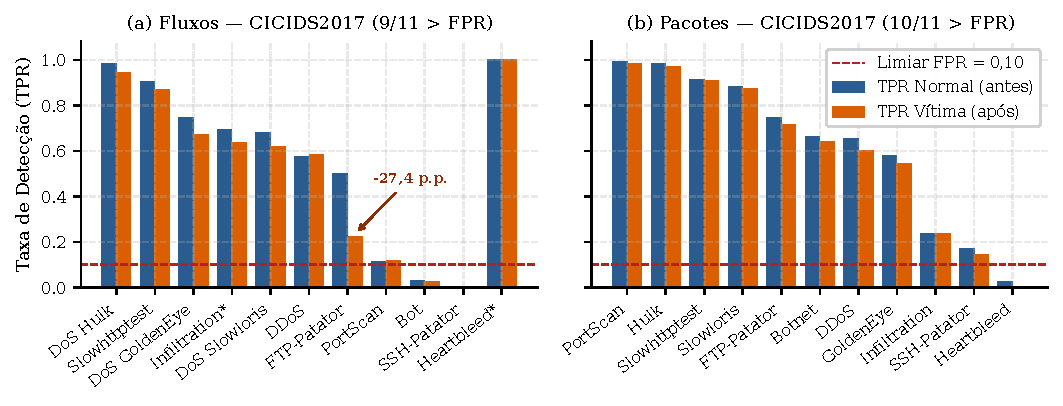
\includegraphics[width=0.92\textwidth]{images/fig_cicids_adversarial.pdf}
\caption{Comparação entre a taxa de detecção antes ($\text{TPR}_{\text{normal}}$) e após ($\text{TPR}_{\text{vítima}}$) os ataques adversariais sob $\text{FPR} = 0{,}10$ no CICIDS2017: (a) fluxos ($8$ de $11$ acima do limiar); e (b) pacotes ($10$ de $11$ acima do limiar). Classes com asterisco possuem suporte reduzido ($n < 100$) em fluxos.}
\label{fig:cicids_adversarial}
\end{figure*}

\begin{table}[!t]
\centering
\footnotesize
\setlength{\tabcolsep}{3.5pt}
\caption{Cenário adversarial em pacotes ($\text{FPR} = 0{,}10$): taxa de detecção antes e depois do ataque e queda condicional por classe.}
\label{tab:adv_pacotes}
\begin{tabular}{@{}lrrrrr@{}}
\toprule
\textbf{Ataque} & \textbf{$n$} & \textbf{TPR norm.} & \textbf{TPR vít.} & \textbf{$\Delta$ (p.p.)} & \textbf{QC} \\
\midrule
Botnet & $9.890$ & $0{,}6653$ & $0{,}6438$ & $-2{,}16$ & $3{,}24\%$ \\
DDoS & $25.000$ & $0{,}6542$ & $0{,}6003$ & $-5{,}39$ & $8{,}24\%$ \\
FTP-Patator & $25.000$ & $0{,}7451$ & $0{,}7157$ & $-2{,}94$ & $3{,}95\%$ \\
DoS GoldenEye & $25.000$ & $0{,}5785$ & $0{,}5435$ & $-3{,}50$ & $6{,}05\%$ \\
Heartbleed & $25.000$ & $0{,}0261$ & $0{,}0001$ & $-2{,}60$ & $99{,}54\%$ \\
DoS Hulk & $25.000$ & $0{,}9832$ & $0{,}9719$ & $-1{,}13$ & $1{,}15\%$ \\
Infiltration & $25.000$ & $0{,}2360$ & $0{,}2354$ & $-0{,}06$ & $0{,}27\%$ \\
PortScan & $25.000$ & $0{,}9913$ & $0{,}9852$ & $-0{,}60$ & $0{,}61\%$ \\
SSH-Patator & $25.000$ & $0{,}1730$ & $0{,}1436$ & $-2{,}94$ & $17{,}00\%$ \\
DoS Slowhttptest & $25.000$ & $0{,}9149$ & $0{,}9096$ & $-0{,}54$ & $0{,}59\%$ \\
DoS slowloris & $25.000$ & $0{,}8822$ & $0{,}8725$ & $-0{,}97$ & $1{,}10\%$ \\
\bottomrule
\end{tabular}
\end{table}

Comparada à granularidade de fluxos, a representação de pacotes é substancialmente mais robusta: a maior queda absoluta é de $5{,}39$ pontos percentuais (DDoS) contra $40{,}74$ em fluxos, e a maior queda condicional entre classes com TPR normal relevante é de $17{,}0\%$ (SSH-Patator) contra $81{,}6\%$.
As maiores quedas absolutas ocorreram em DDoS ($5{,}39$ p.p.), DoS GoldenEye ($3{,}50$ p.p.) e FTP-Patator e SSH-Patator ($2{,}94$ p.p. cada); em Infiltration a queda foi de $0{,}06$ p.p.

A rodada consumiu cerca de $109{,}2$ horas de GPU somadas para $259.890$ amostras.
A execução do laço de $300$ iterações por pacote dentro de um grafo compilado reduziu o tempo de $245{,}1$ s para $94{,}3$ s em um teste A/B controlado de $200$ pacotes, com métricas idênticas ($\text{TPR}_{\text{vítima}} = 0{,}6350$ e três amostras evadidas nos dois modos).

\subsection{Cenário normal sobre o CIC-ToN-IoT}

O CIC-ToN-IoT apresenta um quadro distinto do conjunto de referência (Tabela~\ref{tab:toniot_normal} e Fig.~\ref{fig:new_dataset_comparison}a).
No FPR de $1\%$, o RePO+ atinge média macro de $0{,}2013$ e ponderada de $0{,}0711$, abaixo dos $0{,}2525$ obtidos em fluxos do CICIDS2017; no FPR de $10\%$, os valores sobem para $0{,}6349$ e $0{,}7700$.
Apesar do patamar absoluto mais baixo, a direção do efeito do artigo se reproduz com folga: o ganho do RePO+ sobre o RePO é de $+6{,}28$ pontos percentuais de média macro no FPR de $1\%$ e de $+14{,}35$ pontos no FPR de $10\%$, ambos superiores aos ganhos observados nos dois conjuntos do artigo.
Isso ocorre porque o RePO puro é particularmente frágil neste domínio ($0{,}1384$ de média macro no FPR de $1\%$): como avalia cada fluxo com uma única máscara aleatória, realizações que ocultem os atributos discriminativos do ataque ou que bloqueiem subconjuntos de atributos difíceis de reconstruir no tráfego benigno degradam a separação, enquanto o mínimo por grupo sobre $100$ máscaras no RePO+ filtra máscaras desfavoráveis e recupera a detecção perdida pela observação única.

\begin{table}[!t]
\centering
\footnotesize
\setlength{\tabcolsep}{3.5pt}
\setlength{\tabcolsep}{2.5pt}
\caption{TPR por classe no CIC-ToN-IoT nos pontos de operação de $\text{FPR} = 0{,}01$ e $\text{FPR} = 0{,}10$ (subscritos indicam o FPR alvo).}
\label{tab:toniot_normal}
\begin{tabular}{@{}lrrrrr@{}}
\toprule
\textbf{Classe} & \textbf{$n$} & \textbf{RePO$_{1\%}$} & \textbf{RePO+$_{1\%}$} & \textbf{RePO$_{10\%}$} & \textbf{RePO+$_{10\%}$} \\
\midrule
\textit{backdoor} & $27.145$ & $0{,}3695$ & $0{,}6249$ & $0{,}9945$ & $0{,}9957$ \\
\textit{password} & $340.208$ & $0{,}0415$ & $0{,}1344$ & $0{,}6757$ & $0{,}9697$ \\
\textit{injection} & $277.696$ & $0{,}0278$ & $0{,}0911$ & $0{,}5890$ & $0{,}9221$ \\
\textit{ransomware} & $5.098$ & $0{,}4790$ & $0{,}5947$ & $0{,}7421$ & $0{,}9176$ \\
\textit{xss} & $2.149.308$ & $0{,}0198$ & $0{,}0496$ & $0{,}4554$ & $0{,}7171$ \\
\textit{scanning} & $36.205$ & $0{,}0770$ & $0{,}1135$ & $0{,}5101$ & $0{,}6865$ \\
\textit{mitm} & $517$ & $0{,}2244$ & $0{,}2031$ & $0{,}4371$ & $0{,}5010$ \\
\textit{ddos} & $202$ & $0{,}0000$ & $0{,}0000$ & $0{,}0050$ & $0{,}0050$ \\
\textit{dos} & $145$ & $0{,}0069$ & $0{,}0000$ & $0{,}0138$ & $0{,}0000$ \\
\midrule
Macro & --- & $0{,}1384$ & $0{,}2013$ & $0{,}4914$ & $0{,}6349$ \\
Ponderada & --- & $0{,}0281$ & $0{,}0711$ & $0{,}5012$ & $0{,}7700$ \\
\bottomrule
\end{tabular}
\end{table}

A leitura por classe mostra por que as duas médias divergem tanto.
\textit{backdoor}, \textit{password}, \textit{injection} e \textit{ransomware} são bem detectados no FPR de $10\%$ ($0{,}92$ a $0{,}9957$), enquanto \textit{xss}, que concentra $60\%$ do conjunto de teste, fica em $0{,}7171$ e é o principal limitador da média ponderada.
\textit{ddos} e \textit{dos} praticamente não são detectados em nenhum dos dois pontos de operação, com $202$ e $145$ amostras, respectivamente.
Duas características da avaliação nesse conjunto ajudam a enquadrar esses números.
A primeira é que \textit{ddos} e \textit{dos} têm $202$ e $145$ amostras, de modo que a estimativa é grosseira.
A segunda é que oito dos $77$ atributos apresentam variância nula no conjunto de treinamento benigno e são normalizados apenas pela constante $\epsilon$ da Eq.~\eqref{eq:norm_fluxo} (Seção~\ref{sec:metodologia}); o efeito dessas coordenadas sobre os escores não foi isolado.
Ainda assim, o salto entre os dois pontos de operação é grande (a média macro passa de $0{,}2013$ para $0{,}6349$), o que acompanha a cauda longa da distribuição de escores benignos: baixar o limiar de $0{,}0391$ para $0{,}0070$ triplica o TPR macro.

\begin{figure*}[!t]
\centering
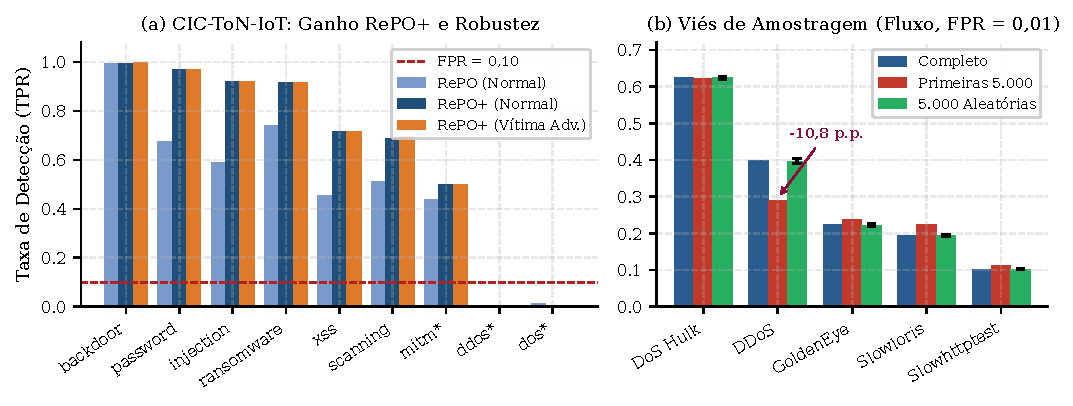
\includegraphics[width=0.92\textwidth]{images/fig_new_dataset_comparison.pdf}
\caption{Generalização e viés de amostragem: (a) RePO vs.\ RePO+ no cenário normal e desempenho pós-ataque (RePO+ Vítima) sob $\text{FPR} = 0{,}10$ no CIC-ToN-IoT; e (b) viés de seleção das primeiras $5.000$ amostras frente ao conjunto completo e à amostragem aleatória ($\pm 1\sigma$) nos fluxos do CICIDS2017 no modo RePO+ sob $\text{FPR} = 0{,}01$.}
\label{fig:new_dataset_comparison}
\end{figure*}

\subsection{Cenário adversarial sobre o CIC-ToN-IoT}

A avaliação adversarial no conjunto adicional atacou $30.864$ amostras em nove classes (Tabela~\ref{tab:toniot_adv} e Fig.~\ref{fig:new_dataset_comparison}a).
O resultado é qualitativamente diferente de tudo o que foi observado no CICIDS2017: houve três evasões em $30.864$ amostras, ou $0{,}010\%$ do total, todas na classe \textit{ransomware}.
O TPR de vítima ponderado é de $0{,}8539$, contra $0{,}8535$ nas mesmas amostras antes do ataque, o que corresponde a um $\Delta$ de $+0{,}04$ ponto percentual; a média macro sobre as nove classes é de $0{,}6354$.
Em sete das nove classes a detecção permaneceu acima do FPR de $10\%$ após o ataque, e as duas exceções (\textit{ddos} e \textit{dos}) já estavam nesse patamar antes de qualquer perturbação.

\begin{table}[!t]
\centering
\footnotesize
\setlength{\tabcolsep}{3.5pt}
\caption{Cenário adversarial no CIC-ToN-IoT ($\text{FPR} = 0{,}10$): detecção antes e depois do ataque por classe ($\dagger$: havia uma única amostra detectada antes do ataque).}
\label{tab:toniot_adv}
\begin{tabular}{@{}lrrrrr@{}}
\toprule
\textbf{Classe} & \textbf{$n$} & \textbf{TPR norm.} & \textbf{TPR vít.} & \textbf{$\Delta$ (p.p.)} & \textbf{QC} \\
\midrule
\textit{backdoor} & $5.000$ & $0{,}9966$ & $0{,}9966$ & $0{,}00$ & $0{,}00\%$ \\
\textit{ransomware} & $5.000$ & $0{,}9172$ & $0{,}9186$ & $+0{,}14$ & $-0{,}15\%$ \\
\textit{password} & $5.000$ & $0{,}9680$ & $0{,}9690$ & $+0{,}10$ & $-0{,}10\%$ \\
\textit{injection} & $5.000$ & $0{,}9202$ & $0{,}9220$ & $+0{,}18$ & $-0{,}20\%$ \\
\textit{xss} & $5.000$ & $0{,}7174$ & $0{,}7180$ & $+0{,}06$ & $-0{,}08\%$ \\
\textit{scanning} & $5.000$ & $0{,}6972$ & $0{,}6954$ & $-0{,}18$ & $+0{,}26\%$ \\
\textit{mitm} & $517$ & $0{,}5010$ & $0{,}4990$ & $-0{,}19$ & $+0{,}39\%$ \\
\textit{ddos} & $202$ & $0{,}0050$ & $0{,}0000$ & $-0{,}50$ & $\dagger$ \\
\textit{dos} & $145$ & $0{,}0000$ & $0{,}0000$ & $0{,}00$ & n/d \\
\bottomrule
\end{tabular}
\end{table}

A primeira explicação para esse contraste é que a taxa de sucesso aparente do ataque engana neste conjunto.
$14{,}6\%$ das amostras atacadas já eram classificadas como benignas antes de qualquer otimização, e a diferença $1 - \text{TPR}_{\text{vítima}}$ contabiliza integralmente esses falsos negativos preexistentes.
A queda condicional, que desconta esse efeito, fica em $0{,}00\%$ para \textit{backdoor}, $0{,}26\%$ para \textit{scanning} e $0{,}39\%$ para \textit{mitm}, ou seja, no limite do ruído de reavaliação observado no próprio conjunto.
Na classe \textit{ddos}, a queda condicional de $100\%$ indicada por $\dagger$ corresponde a uma única amostra: havia uma detecção entre $202$ amostras e ela deixou de ocorrer; em \textit{dos} o denominador é zero e a métrica não é definida.
Reportar esses dois casos como evidência de eficácia do ataque seria um artefato de denominador.

A segunda explicação é estrutural e diz respeito ao desalinhamento entre o objetivo do atacante e a métrica de sucesso.
A perda otimizada pelo ataque é a média dos $100$ erros de reconstrução, enquanto o escore que decide a detecção é o RePO+, isto é, a soma dos mínimos por grupo.
Reduzir a média não reduz necessariamente o mínimo: basta que algumas máscaras continuem reconstruindo bem a amostra modificada para que o escore agregado permaneça alto.
Essa é a hipótese mais provável apontada na análise deste conjunto para a assimetria entre “amostra modificada com sucesso” e “amostra que evade” — consistente com os dados, mas não demonstrada, pois testá-la exigiria medir o erro por máscara antes e depois do ataque.
Sob essa leitura, as três evasões em trinta mil amostras indicam ausência de efeito mensurável, e não um ataque que \emph{funciona pouco}.
O custo dessa rodada foi de $31{,}4$ horas de parede e $62{,}5$ horas de GPU, o que corresponde a $7{,}29$ segundos por amostra.

\subsection{Discussão comparativa entre granularidades e domínios}

A Tabela~\ref{tab:comparativo} reúne os três blocos experimentais.
A comparação mais informativa é a queda condicional, porque ela desconta os falsos negativos que já existiam: o pior ataque de fluxo do CICIDS2017 suprime $81{,}6\%$ das detecções existentes, o pior ataque de pacotes com TPR normal relevante fica em $17{,}0\%$ e o pior caso no CIC-ToN-IoT em $0{,}39\%$.
Como são conjuntos de dados diferentes, essa comparação é descritiva e não uma medida de generalização estatística.

\begin{table*}[!t]
\centering
\footnotesize
\setlength{\tabcolsep}{8pt}
\caption{Síntese comparativa dos três blocos adversariais avaliados.}
\label{tab:comparativo}
\begin{tabular}{@{}lrrr@{}}
\toprule
\textbf{Métrica} & \textbf{Fluxos (CICIDS2017)} & \textbf{Pacotes (CICIDS2017)} & \textbf{Fluxos (CIC-ToN-IoT)} \\
\midrule
Amostras atacadas & $47.003$ & $259.890$ & $30.864$ \\
Classes de ataque & $11$ & $11$ & $9$ \\
TPR de vítima ponderado & $0{,}4663$ & $0{,}5995$ & $0{,}8539$ \\
TPR de vítima macro & $0{,}5059$ & $0{,}6020$ & $0{,}6354$ \\
Maior queda absoluta (p.p.) & $-40{,}74$ & $-5{,}39$ & $-0{,}50$ \\
Maior queda condicional & $81{,}6\%$ & $17{,}0\%$ & $0{,}39\%$ \\
Classes acima do FPR após o ataque & $8$ de $11$ & $10$ de $11$ & $7$ de $9$ \\
Custo por amostra & $\approx 1{,}16$ s & $\approx 1{,}0$ s & $7{,}29$ s \\
\bottomrule
\end{tabular}
\end{table*}

Essa diferença pede cautela: mudam o conjunto de dados, as features, a escala dos escores e o próprio limiar.
Em fluxos do CICIDS2017 o atacante otimiza contra $0{,}8\tau$ para compensar a substituição de máscaras, em pacotes ele opera no limiar publicado e no conjunto adicional o limiar é recalibrado no próprio conjunto, de modo que os três blocos não operam no mesmo ponto de operação.
Quanto à resolução das medidas, no conjunto adicional as diferenças entre o antes e o depois são da ordem de $\pm 0{,}2$ ponto percentual e, em quatro das nove classes, o TPR chegou a aumentar; no fluxo do CICIDS2017, PortScan e DDoS também apresentaram TPR superior após o ataque.

Uma ressalva adicional diz respeito à ponderação no conjunto adicional: o TPR de vítima ponderado ($0{,}8539$) é medido sobre no máximo $5.000$ amostras por classe, enquanto \textit{xss} tem $2{,}15$ milhões de amostras no conjunto de teste completo, de modo que a ponderação da rodada adversarial não é a mesma da avaliação normal.

Quanto à comparação com outros trabalhos, a reprodução preserva a ordenação qualitativa defendida no artigo: o RePO+ supera o RePO nos três conjuntos avaliados, e os valores absolutos do cenário normal ficam a menos de meio ponto percentual dos publicados.
Como os detectores concorrentes (Kitsune, DAGMM e BiGAN) não foram retreinados neste trabalho, a comparação com eles permanece a reportada pelos autores originais, discutida na Seção~\ref{sec:sistema_referencia} e sintetizada na Tabela~\ref{tab:trabalhos-relacionados}; o que esta replicação acrescenta é a verificação de que a ordenação qualitativa do artigo se mantém nos três conjuntos avaliados.

Por fim, as limitações que afetam a leitura dos números são as seguintes: as classes minoritárias do CICIDS2017 (Heartbleed, com $11$ fluxos, e Infiltration, com $36$) têm intervalos de confiança largos e foram mantidas nas médias macro por fidelidade ao protocolo; a seleção das primeiras $N$ amostras por classe introduz viés temporal, com o DDoS caindo de $0{,}3177$ para $0{,}1898$ no RePO e de $0{,}3974$ para $0{,}2890$ no RePO+; a reavaliação com uma única amostragem de máscaras limita a resolução a cerca de um ponto percentual; e a calibração do limiar adversarial em fluxos depende de um fator $0{,}8$ empírico, que funciona nos dados avaliados mas não é derivado de um princípio e exigiria recalibração em um modelo retreinado.

\subsection{Proposta 1: cascata cheap-first}

A Tabela~\ref{tab:cascata_normal} apresenta o custo e a acurácia das nove configurações de cascata avaliadas, além do detector de referência e da decisão sequencial.
O resultado central é que as nove configurações têm a mesma TPR do RePO+ completo da mesma rodada ($0{,}2560$ de média macro e $0{,}1871$ ponderada, idênticas até a sexta casa decimal), com o mesmo $\text{FPR}$ de $1\%$ e o mesmo limiar final.
Não há ganho de acurácia; há ganho de custo, e ele vem de o limiar final ser calibrado sobre o escore cascateado e de nenhuma amostra descartada ter sido detectada.
O melhor ponto da grade é o estágio barato com $10$ máscaras e orçamento de $1\%$ de falsos negativos: $60{,}80$ máscaras por amostra, redução de $39{,}2\%$ em relação às $100$, com $43{,}98\%$ dos benignos resolvidos pelo atalho.

\begin{table*}[!t]
\centering
\footnotesize
\setlength{\tabcolsep}{6pt}
\caption{Custo e acurácia da cascata cheap-first e da decisão sequencial na mistura de avaliação ($99\%$ benigno / $1\%$ ataque), $\text{FPR} = 1\%$. A coluna de falsos negativos é a fração medida do orçamento do atalho.}
\label{tab:cascata_normal}
\begin{tabular}{@{}lrrrrrr@{}}
\toprule
\textbf{Regra} & \textbf{TPR macro} & \textbf{TPR pond.} & \textbf{Máscaras/am.} & \textbf{Ganho} & \textbf{Benignos pulados} & \textbf{FN medido} \\
\midrule
Média simples ($100$ máscaras) & $0{,}2396$ & $0{,}1581$ & $100{,}00$ & --- & --- & --- \\
RePO+ (artigo, 100 máscaras) & $0{,}2546$ & $0{,}1873$ & $100{,}00$ & --- & --- & --- \\
RePO+ (referência interna, 5 rep.) & $0{,}2560$ & $0{,}1871$ & $100{,}00$ & --- & $0{,}00\%$ & $0{,}00\%$ \\
\midrule
cascata $n_{\text{cheap}}=5$, FN $0$ & $0{,}2560$ & $0{,}1871$ & $72{,}66$ & $27{,}3\%$ & $29{,}07\%$ & $0{,}00\%$ \\
cascata $n_{\text{cheap}}=5$, FN $0{,}1\%$ & $0{,}2560$ & $0{,}1871$ & $67{,}42$ & $32{,}6\%$ & $34{,}64\%$ & $0{,}10\%$ \\
cascata $n_{\text{cheap}}=5$, FN $1\%$ & $0{,}2560$ & $0{,}1871$ & $64{,}83$ & $35{,}2\%$ & $37{,}39\%$ & $1{,}00\%$ \\
cascata $n_{\text{cheap}}=10$, FN $0$ & $0{,}2560$ & $0{,}1871$ & $66{,}37$ & $33{,}6\%$ & $37{,}74\%$ & $0{,}00\%$ \\
cascata $n_{\text{cheap}}=10$, FN $0{,}1\%$ & $0{,}2560$ & $0{,}1871$ & $64{,}04$ & $36{,}0\%$ & $40{,}36\%$ & $0{,}10\%$ \\
\textbf{cascata $n_{\text{cheap}}=10$, FN $1\%$} & $\mathbf{0{,}2560}$ & $\mathbf{0{,}1871}$ & $\mathbf{60{,}80}$ & $\mathbf{39{,}2\%}$ & $\mathbf{43{,}98\%}$ & $\mathbf{1{,}00\%}$ \\
cascata $n_{\text{cheap}}=25$, FN $0$ & $0{,}2560$ & $0{,}1871$ & $80{,}81$ & $19{,}2\%$ & $25{,}85\%$ & $0{,}00\%$ \\
cascata $n_{\text{cheap}}=25$, FN $0{,}1\%$ & $0{,}2560$ & $0{,}1871$ & $69{,}83$ & $30{,}2\%$ & $40{,}63\%$ & $0{,}10\%$ \\
cascata $n_{\text{cheap}}=25$, FN $1\%$ & $0{,}2560$ & $0{,}1871$ & $68{,}84$ & $31{,}2\%$ & $41{,}96\%$ & $1{,}00\%$ \\
\midrule
RePO sequencial (blocos de 5) & $0{,}2438$ & $0{,}1577$ & $\mathbf{5{,}32}$ & $\mathbf{94{,}7\%}$ & --- & --- \\
\bottomrule
\end{tabular}
\end{table*}

Três propriedades qualificam esse resultado.
A primeira é que o ponto ótimo não está nos extremos da grade: com $5$ máscaras o escore barato é mais ruidoso, o $t_{\text{low}}$ calibrado sobe e menos benignos pulam ($37{,}39\%$ contra $43{,}98\%$); com $25$ máscaras o estágio barato é caro e o limiar fica tão baixo que apenas $41{,}96\%$ pulam.
A economia máxima é, portanto, um compromisso entre o custo do prefixo e a seletividade do atalho.
A segunda é que o orçamento de falsos negativos é consumido exatamente: $1\%$ de $44.182$ ataques corresponde a $442$ amostras, e o valor medido é $1{,}0004\%$.
A terceira é que a diferença entre o RePO+ de $100$ máscaras do artigo ($0{,}2546$) e a referência interna com cinco repetições ($0{,}2560$) é de $0{,}0013$, compatível com o desvio entre repetições ($\approx 0{,}0011$); ela é a média de cinco sorteios contra um, e não uma mudança de comportamento do detector.

\begin{table*}[!t]
\centering
\footnotesize
\setlength{\tabcolsep}{6pt}
\caption{Avaliação adversarial da cascata: TPR antes e depois do ataque e taxa de contorno do estágio barato, no ponto de operação de $\text{FPR} \approx 10\%$, com $1.000$ amostras por ataque.}
\label{tab:cascata_adv}
\begin{tabular}{@{}lrrrrrrr@{}}
\toprule
& & \multicolumn{2}{c}{\textbf{$n_{\text{cheap}} = 5$}} & \multicolumn{2}{c}{\textbf{$n_{\text{cheap}} = 10$}} & \multicolumn{2}{c}{\textbf{$n_{\text{cheap}} = 25$}} \\
\cmidrule(lr){3-4}\cmidrule(lr){5-6}\cmidrule(l){7-8}
\textbf{Ataque} & \textbf{$n$} & \textbf{TPR vít.} & \textbf{bypass} & \textbf{TPR vít.} & \textbf{bypass} & \textbf{TPR vít.} & \textbf{bypass} \\
\midrule
FTP-Patator & $1.000$ & $0{,}504$ & $0{,}0\%$ & $0{,}499$ & $0{,}0\%$ & $0{,}502$ & $0{,}1\%$ \\
SSH-Patator & $1.000$ & $0{,}006$ & $5{,}3\%$ & $0{,}006$ & $2{,}0\%$ & $0{,}006$ & $0{,}0\%$ \\
DoS slowloris & $1.000$ & $0{,}664$ & $0{,}0\%$ & $0{,}665$ & $0{,}0\%$ & $0{,}665$ & $0{,}0\%$ \\
DoS Slowhttptest & $1.000$ & $0{,}932$ & $0{,}0\%$ & $0{,}932$ & $0{,}0\%$ & $0{,}932$ & $0{,}0\%$ \\
DoS Hulk & $1.000$ & $0{,}991$ & $0{,}0\%$ & $0{,}991$ & $0{,}0\%$ & $0{,}991$ & $0{,}0\%$ \\
DoS GoldenEye & $1.000$ & $0{,}719$ & $0{,}0\%$ & $0{,}719$ & $0{,}0\%$ & $0{,}719$ & $0{,}0\%$ \\
Heartbleed & $11$ & $1{,}000$ & $0{,}0\%$ & $1{,}000$ & $0{,}0\%$ & $1{,}000$ & $0{,}0\%$ \\
Infiltration & $36$ & $0{,}667$ & $0{,}0\%$ & $0{,}667$ & $2{,}8\%$ & $0{,}667$ & $0{,}0\%$ \\
Bot & $1.000$ & $0{,}029$ & $0{,}7\%$ & $0{,}029$ & $0{,}2\%$ & $0{,}029$ & $0{,}1\%$ \\
PortScan & $1.000$ & $0{,}117$ & $0{,}0\%$ & $0{,}117$ & $0{,}0\%$ & $0{,}117$ & $0{,}0\%$ \\
DDoS & $1.000$ & $0{,}641$ & $0{,}0\%$ & $0{,}641$ & $0{,}0\%$ & $0{,}641$ & $0{,}0\%$ \\
\midrule
\textbf{Agregado} & $\mathbf{9.047}$ & --- & $\mathbf{0{,}663\%}$ & --- & $\mathbf{0{,}254\%}$ & --- & $\mathbf{0{,}022\%}$ \\
\bottomrule
\end{tabular}
\end{table*}

A Tabela~\ref{tab:cascata_adv} reporta o ataque ao estágio barato em $9.047$ amostras.
A taxa de contorno agregada é de $0{,}663\%$ com $5$ máscaras, $0{,}254\%$ com $10$ (intervalo de Wilson de $95\%$: $0{,}169$–$0{,}381\%$) e $0{,}022\%$ com $25$.
Como $t_{\text{low}}$ é cerca de $60$ vezes menor que o limiar de decisão no caso de $10$ máscaras, todo escore abaixo dele também está abaixo de $\tau$; o contorno é, portanto, um \emph{limite inferior} da evasão, e não a taxa de evasão.
Duas ressalvas de leitura acompanham o número: contornar o estágio barato não é o mesmo que perder a detecção (PortScan e Slowhttptest têm onze detecções perdidas com contorno nulo, ou seja, a perda ocorreu no escore completo e não no atalho), e parte das amostras já era falso negativo antes de qualquer otimização (SSH-Patator: $993$ de $1.000$; Bot: $971$; PortScan: $888$).
Excluindo o SSH-Patator, cujo TPR no ponto de operação é de $0{,}007$ e cujo contorno mede, portanto, cegueira preexistente (havia uma única detecção para perder, e ela foi contabilizada), o contorno agregado cai para $0{,}09\%$, $0{,}04\%$ e $0{,}02\%$ nas três configurações.
Em Infiltration o contorno de $2{,}8\%$ com $10$ máscaras corresponde a um único evento em $36$ amostras, cujo intervalo de confiança de Wilson vai de $0{,}5\%$ a $14{,}2\%$.
Vale registrar ainda que as TPRs dessa tabela são medidas no ponto de operação de $10\%$ de FPR e não correspondem à operação a $1\%$: no baseline, FTP-Patator tem TPR $0{,}0000$, SSH-Patator $0{,}0002$ e PortScan $0{,}0000$ nesse ponto.

\begin{table}[!t]
\centering
\footnotesize
\setlength{\tabcolsep}{4pt}
\caption{Sensibilidade do custo da cascata ($n_{\text{cheap}}=10$, FN $1\%$) à prevalência de ataque.}
\label{tab:prevalencia}
\begin{tabular}{@{}llrr@{}}
\toprule
\textbf{$p_{\text{ben}}$ / $p_{\text{atk}}$} & \textbf{$f_{\text{roteada}}$} & \textbf{Máscaras/am.} & \textbf{Ganho} \\
\midrule
$100\%$ / $0\%$ & $0{,}560$ & $60{,}42$ & $39{,}6\%$ \\
$99\%$ / $1\%$ (avaliação) & $0{,}564$ & $60{,}80$ & $39{,}2\%$ \\
$90\%$ / $10\%$ & $0{,}603$ & $64{,}28$ & $35{,}7\%$ \\
$50\%$ / $50\%$ & $0{,}775$ & $79{,}76$ & $20{,}2\%$ \\
$10\%$ / $90\%$ & $0{,}947$ & $95{,}23$ & $4{,}8\%$ \\
$0\%$ / $100\%$ & $0{,}990$ & $99{,}10$ & $0{,}9\%$ \\
\bottomrule
\end{tabular}
\end{table}

A economia é dependente da carga, como a Eq.~\eqref{eq:custo_cascata} prevê (Tabela~\ref{tab:prevalencia}).
Com $100\%$ de tráfego benigno o custo cai para $60{,}42$ máscaras por amostra; com metade de ataque, o ganho recua para $20{,}2\%$; com tráfego inteiramente hostil, a redução de custo é de apenas $0{,}9\%$, porque o orçamento de falsos negativos impede que ataques pulem o ensemble.
O valor agregado só tem significado acompanhado da prevalência em que foi medido.

\subsection{Proposta 2: decisão sequencial}

A decisão sequencial leva o custo a $5{,}32$ máscaras por amostra (redução de $94{,}7\%$), mantendo $99{,}93\%$ de concordância com a decisão pela média de $100$ máscaras e um FPR de $0{,}9916\%$, ligeiramente abaixo do alvo porque o intervalo de confiança às vezes decide "benigno" antes de a média cruzar o limiar.
Contudo, o preço aparece na acurácia: a TPR macro é de $0{,}2438$ e a ponderada de $0{,}1577$, contra $0{,}2560$ e $0{,}1871$ do RePO+ — uma perda de $1{,}2$ ponto percentual na média macro e de $2{,}9$ pontos na ponderada.
Parte dessa diferença é a troca de detector: a regra sequencial opera sobre a média amostral dos erros por máscara e não sobre o RePO+, porque é a média que admite estimador de intervalo; a referência comparativa é o escore médio sobre $100$ máscaras, e como a regra decide o mesmo em $99{,}93\%$ dos casos, a TPR realizada fica a uma fração de ponto percentual desse valor.
A avaliação adversarial dessa regra ainda não foi concluída: o ataque foi especificado e implementado para otimizar a estatística que a regra usa (o limite superior do intervalo do primeiro bloco), mas a execução estava em andamento no fechamento desta versão, de modo que a comparação direta entre as duas propostas permanece aberta.

\subsection{Síntese: custo $\times$ robustez das duas propostas}

A Tabela~\ref{tab:custo_robustez} coloca as duas propostas lado a lado com o detector de referência.
O resultado é consistente entre as duas propostas: a cascata reduz o custo ao preço de uma superfície de ataque nova, que é pequena no protocolo medido; a decisão sequencial reduz o custo em maior grau, mas troca de detector e ainda não foi atacada.
Do ponto de vista de recomendação, o estágio barato de $10$ máscaras com orçamento de $1\%$ de falsos negativos é o ponto defensável da grade (é o menor custo medido, preserva a TPR do artigo e mantém a taxa de contorno agregada abaixo de $0{,}3\%$), com a ressalva de que qualquer afirmação sobre economia precisa vir acompanhada da prevalência (Tabela~\ref{tab:prevalencia}).

\begin{table}[!t]
\centering
\footnotesize
\setlength{\tabcolsep}{4pt}
\caption{Comparação final entre o detector de referência e as duas propostas.}
\label{tab:custo_robustez}
\begin{tabular}{@{}lrrr@{}}
\toprule
\textbf{Regra} & \textbf{Máscaras/am.} & \textbf{TPR macro} & \textbf{Bypass} \\
\midrule
RePO+ ($100$ máscaras) & $100{,}00$ & $0{,}2560$ & --- \\
cascata $10$/FN $0$ & $66{,}37$ & $0{,}2560$ & não medido \\
cascata $10$/FN $1\%$ & $60{,}80$ & $0{,}2560$ & $0{,}25\%$ \\
cascata $25$/FN $1\%$ & $68{,}84$ & $0{,}2560$ & $0{,}02\%$ \\
sequencial (blocos de $5$) & $5{,}32$ & $0{,}2438$ & não avaliado \\
\bottomrule
\end{tabular}
\end{table}

\section{Conclusões e trabalhos futuros}

Este trabalho reproduziu o método RePO/RePO+ com alta fidelidade nos dados do artigo ($0{,}2525$ de TPR em fluxos e $0{,}3472$ em pacotes no cenário normal, contra $0{,}2549$ e $0{,}3477$ publicados), auditou o protocolo de avaliação, identificando o viés da seleção sequencial de amostras, o ruído da reavaliação com máscara única e o peso das classes minoritárias, e estendeu a avaliação a um conjunto de tráfego de Internet das Coisas, no qual a vantagem do RePO+ sobre o RePO se mantém e o ataque adversarial se mostra ineficaz.
Sobre essa base, a contribuição que o trabalho defende é de outra natureza: \textbf{o gargalo de implantação de um detector como o RePO+ não é a acurácia, e sim o custo}.

O detector RePO+ de referência gasta $100$ passagens pelo autoencoder por amostra, porque o escore é calculado a partir de um ensemble de $100$ erros de reconstrução, e esse custo cresce linearmente com o número de máscaras.
As duas propostas avaliadas atacam esse custo pela alocação de máscaras por amostra, e não pela redução uniforme do orçamento: a amostra que não usa o atalho continua sendo julgada pelo mesmo RePO+ de $100$ máscaras do artigo.
A cascata \textit{cheap-first} com estágio barato de $10$ máscaras e orçamento de $1\%$ de falsos negativos reduz o custo de $100$ para $60{,}80$ máscaras por amostra ($-39{,}2\%$) na mistura de avaliação, resolve $43{,}98\%$ do tráfego benigno com $10$ máscaras, preserva exatamente a TPR do RePO+ completo ($0{,}2560$ macro e $0{,}1871$ ponderada, com o mesmo $\text{FPR}$ de $1\%$ e o mesmo limiar) e apresenta taxa de contorno agregada de $0{,}25\%$ sob ataque — $0{,}04\%$ quando se exclui o SSH-Patator, cujo contorno mede cegueira preexistente do detector.
A decisão sequencial, que revela máscaras em blocos de cinco e para quando o intervalo de confiança exclui o limiar, leva o custo a $5{,}32$ máscaras por amostra ($-94{,}7\%$) com $99{,}93\%$ de concordância com a decisão completa, ao preço de $1{,}2$ ponto percentual de TPR macro e da troca do agregador do RePO+ pela média amostral dos erros por máscara.

Os dois resultados sustentam a conclusão de que \textbf{reduzir custo sem degradar a decisão é possível quando o orçamento computacional é alocado por amostra}, e de que essa redução é mensurável, mas não é universal.
Ela é mensurável porque a cascata preserva a função de decisão na região em que ela importa e porque o custo por amostra pode ser contabilizado com precisão — $60{,}80$ máscaras na mistura avaliada, com o orçamento de falsos negativos consumido exatamente ($1{,}0004\%$ de $44.182$ ataques).
Ela não é universal porque só amostras benignas podem ser descartadas: o mesmo detector custa $60{,}42$ máscaras por amostra em tráfego exclusivamente benigno, $79{,}76$ em uma carga com metade de ataques e $99{,}10$ em tráfego inteiramente hostil.
Qualquer afirmação sobre economia precisa, portanto, vir acompanhada da prevalência de ataque em que foi medida.

O que os dados permitem afirmar e o que não permitem também delimita o trabalho.
Não se pode afirmar que a cascata seja mais robusta que o RePO+: ela acrescenta um caminho de decisão que antes não existia, e o ataque a esse caminho é possível em princípio — o que se mediu foi uma superfície pequena no protocolo avaliado, não a ausência de superfície.
Não se pode afirmar que $60{,}80$ seja um número transferível: o limiar do estágio barato é calibrado nos mesmos ataques que depois são avaliados, de modo que a garantia de falsos negativos é in-sample e pode ser consumida de outra forma em uma população de ataques diferente.
E não se pode fechar a comparação entre as duas propostas, porque a decisão sequencial troca o detector e ainda não foi submetida ao ataque adversarial.

As limitações do estudo acompanham essas ressalvas: a avaliação cobre um único conjunto de dados e uma única arquitetura, com $1.000$ amostras por ataque no cenário adversarial, das quais duas classes têm $11$ e $36$ amostras e, portanto, nenhuma taxa estimável com precisão; o ponto de operação adversarial é o de $10\%$ de FPR, mais permissivo que a operação a $1\%$; e a cascata não foi avaliada na granularidade de pacotes.
Os trabalhos futuros seguem diretamente dessas lacunas: concluir o ataque à decisão sequencial e compará-la à cascata no mesmo protocolo; construir uma versão sequencial do RePO+, que exige um estimador de intervalo para a soma de mínimos por grupo, e não apenas para a média; avaliar a cascata em pacotes; e incorporar a prevalência como parâmetro explícito de projeto, já que a economia depende dela.
Duas direções investigadas em paralelo permanecem como candidatas a combinar com a alocação por amostra: as máscaras estruturadas, que reduzem o orçamento de base sem alterar a decisão na região difícil, e a destilação, que reduz o custo por avaliação mas, nos pilotos realizados, não preservou a robustez adversarial.

\begin{thebibliography}{99}

\bibitem{symantec2019}
Symantec, ``Internet security threat report,'' Symantec Corporation, Tech. Rep., 2019.

\bibitem{icscert2016}
ICS-CERT, ``Cyber-attack against Ukrainian critical infrastructure,'' Industrial Control Systems Cyber Emergency Response Team, Alert IR-ALERT-H-16-056-01, 2016.

\bibitem{kumar2017}
R.~S.~S. Kumar, A.~Wicker, and M.~Swann, ``Practical machine learning for cloud intrusion detection: Challenges and the way forward,'' in \emph{Proc. 10th ACM Workshop on Artificial Intelligence and Security (AISec)}, Dallas, TX, USA, 2017, pp. 81--90.

\bibitem{ahmad2015}
I.~Ahmad, S.~Namal, M.~Ylianttila, and A.~Gurtov, ``Security in software defined networks: A survey,'' \emph{IEEE Communications Surveys \& Tutorials}, vol.~17, no.~4, pp. 2317--2346, 2015.

\bibitem{lee2017}
S.~Lee, J.~Kim, S.~Shin, P.~Porras, and V.~Yegneswaran, ``Athena: A framework for scalable anomaly detection in software-defined networks,'' in \emph{Proc. 47th Annual IEEE/IFIP Int. Conf. on Dependable Systems and Networks (DSN)}, Denver, CO, USA, 2017, pp. 249--260.

\bibitem{khraisat2019}
A.~Khraisat, I.~Gondal, P.~Vamplew, and J.~Kamruzzaman, ``Survey of intrusion detection systems: Techniques, datasets and challenges,'' \emph{Cybersecurity}, vol.~2, no.~1, pp. 1--22, 2019.

\bibitem{alqatf2018}
M.~Al-Qatf, Y.~Lasheng, M.~Al-Habib, and K.~Al-Sabahi, ``Deep learning approach combining sparse autoencoder with SVM for network intrusion detection,'' \emph{IEEE Access}, vol.~6, pp. 52\,843--52\,856, 2018.

\bibitem{yu2017}
Y.~Yu, J.~Long, and Z.~Cai, ``Network intrusion detection through stacking dilated convolutional autoencoders,'' \emph{Security and Communication Networks}, vol. 2017, pp. 1--10, 2017.

\bibitem{yin2018}
C.~Yin, Y.~Zhu, S.~Liu, J.~Fei, and H.~Zhang, ``An enhancing framework for botnet detection using generative adversarial networks,'' in \emph{Proc. Int. Conf. on Artificial Intelligence and Big Data (ICAIBD)}, Chengdu, China, 2018, pp. 228--234.

\bibitem{malaiya2018}
R.~K. Malaiya, D.~Kwon, J.~Kim, S.~C. Suh, H.~Kim, and I.~Kim, ``An empirical evaluation of deep learning for network anomaly detection,'' in \emph{Proc. Int. Conf. on Computing, Networking and Communications (ICNC)}, Maui, HI, USA, 2018, pp. 893--898.

\bibitem{mirsky2018}
Y.~Mirsky, T.~Doitshman, Y.~Elovici, and A.~Shabtai, ``Kitsune: An ensemble of autoencoders for online network intrusion detection,'' in \emph{Proc. Network and Distributed System Security Symposium (NDSS)}, San Diego, CA, USA, 2018, pp. 1--15.

\bibitem{zong2018}
B.~Zong, Q.~Song, M.~R. Min, W.~Cheng, C.~Lumezanu, D.~Cho, and H.~Chen, ``Deep autoencoding Gaussian mixture model for unsupervised anomaly detection,'' in \emph{Proc. Int. Conf. on Learning Representations (ICLR)}, Vancouver, BC, Canada, 2018, pp. 1--19.

\bibitem{zenati2018}
H.~Zenati, C.~S. Foo, B.~Lecouat, G.~Manek, and V.~R. Chandrasekhar, ``Efficient GAN-based anomaly detection,'' \emph{arXiv preprint arXiv:1802.06222}, 2018.

\bibitem{chalapathy2019}
R.~Chalapathy and S.~Chawla, ``Deep learning for anomaly detection: A survey,'' \emph{arXiv preprint arXiv:1901.03407}, 2019.

\bibitem{hashemi2019}
M.~J. Hashemi, G.~Cusack, and E.~Keller, ``Towards evaluation of NIDSs in adversarial setting,'' in \emph{Proc. 3rd ACM CoNEXT Workshop on Big DAta, Machine Learning and Artificial Intelligence for Data Communication Networks (Big-DAMA)}, Orlando, FL, USA, 2019, pp. 14--21.

\bibitem{aiken2019}
J.~Aiken and S.~Scott-Hayward, ``Investigating adversarial attacks against network intrusion detection systems in SDNs,'' in \emph{Proc. IEEE Conf. on Network Function Virtualization and Software Defined Networks (NFV-SDN)}, Dallas, TX, USA, 2019, pp. 1--7.

\bibitem{hashemi2020}
M.~J. Hashemi and E.~Keller, ``Enhancing robustness against adversarial examples in network intrusion detection systems,'' in \emph{Proc. IEEE Conf. on Network Function Virtualization and Software Defined Networks (NFV-SDN)}, Leganés, Spain, 2020, pp. 1--7.

\bibitem{vincent2008}
P.~Vincent, H.~Larochelle, Y.~Bengio, and P.-A. Manzagol, ``Extracting and composing robust features with denoising autoencoders,'' in \emph{Proc. 25th Int. Conf. on Machine Learning (ICML)}, Helsinki, Finland, 2008, pp. 1096--1103.

\bibitem{biggio2013}
B.~Biggio, I.~Corona, D.~Maiorca, B.~Nelson, N.~{\v{S}}rndi{\fontencoding{OT1}\selectfont\'c}, P.~Laskov, G.~Giacinto, and F.~Roli, ``Evasion attacks against machine learning at test time,'' in \emph{Proc. European Conf. on Machine Learning and Knowledge Discovery in Databases (ECML PKDD)}, Prague, Czech Republic, 2013, pp. 387--402.

\bibitem{szegedy2013}
C.~Szegedy, W.~Zaremba, I.~Sutskever, J.~Bruna, D.~Erhan, I.~Goodfellow, and R.~Fergus, ``Intriguing properties of neural networks,'' \emph{arXiv preprint arXiv:1312.6199}, 2013.

\bibitem{carlini2018}
N.~Carlini and D.~Wagner, ``Audio adversarial examples: Targeted attacks on speech-to-text,'' in \emph{Proc. IEEE Security and Privacy Workshops (SPW)}, San Francisco, CA, USA, 2018, pp. 1--7.

\bibitem{sharif2016}
M.~Sharif, S.~Bhagavatula, L.~Bauer, and M.~K. Reiter, ``Accessorize to a crime: Real and stealthy attacks on state-of-the-art face recognition,'' in \emph{Proc. ACM SIGSAC Conf. on Computer and Communications Security (CCS)}, Vienna, Austria, 2016, pp. 1528--1540.

\bibitem{eykholt2018}
K.~Eykholt, I.~Evtimov, E.~Fernandes, B.~Li, A.~Rahmati, C.~Xiao, A.~Prakash, T.~Kohno, and D.~Song, ``Robust physical-world attacks on deep learning visual classification,'' in \emph{Proc. IEEE/CVF Conf. on Computer Vision and Pattern Recognition (CVPR)}, Salt Lake City, UT, USA, 2018, pp. 1625--1634.

\bibitem{grosse2017}
K.~Grosse, N.~Papernot, P.~Manoharan, M.~Backes, and P.~McDaniel, ``Adversarial examples for malware detection,'' in \emph{Proc. 22nd European Symposium on Research in Computer Security (ESORICS)}, Oslo, Norway, 2017, pp. 62--79.

\bibitem{sharafaldin2018}
I.~Sharafaldin, A.~H. Lashkari, and A.~A. Ghorbani, ``Toward generating a new intrusion detection dataset and intrusion traffic characterization,'' in \emph{Proc. 4th Int. Conf. on Information Systems Security and Privacy (ICISSP)}, Funchal, Madeira, Portugal, 2018, pp. 108--116.

\bibitem{axelsson2000}
S.~Axelsson, ``The base-rate fallacy and the difficulty of intrusion detection,'' \emph{ACM Transactions on Information and System Security (TISSEC)}, vol.~3, no.~3, pp. 186--205, 2000.

\bibitem{sarhan2022cictoniot}
M.~Sarhan, S.~Layeghy, and M.~Portmann, ``Evaluating standard feature sets towards increased generalisability and explainability of ML-based network intrusion detection,'' \emph{Big Data Research}, vol.~30, p. 100359, 2022.

\bibitem{moustafa2019toniot}
N.~Moustafa, ``ToN-IoT datasets,'' \emph{IEEE DataPort}, 2019, doi: 10.21227/fesz-dm97.

\end{thebibliography}

\end{document}
